\subsection{Three Dimensional Plot Types}
{
\tikzset{external/figure name/.add={}{threedim_}}%
\label{sec:3d}
\PGFPlots\ provides three dimensional visualizations like scatter, line, mesh or surface plots. This section explains the methods to provide input coordinates and how to use the different plot types.

\subsubsection{Before You Start With 3D}
\label{pgfplots:3d:preliminary}
Before we delve into the capabilities of \PGFPlots\ for three dimensional visualization, let me start with some preliminary remarks. The reason to use \PGFPlots\ for three dimensional plots are similar to those of normal, two dimensional plots: the possibility to get consistent fonts and document consistent styles combined with high--quality output.

While this works very nice for (not too complex) two dimensional plots, it requires considerably more effort than non--graphical documents. This is even more so for three dimensional plots. In other words: \PGFPlots' three dimensional routines are slow. There are reasons for this and some of them may vanish in future versions. But one of these reasons is that \TeX\ has never been designed for complex visualisation techniques. Consider the image externalization routines mentioned in Section~\ref{sec:pgfplots:export}, in particular the |external| library to reduce typesetting time. Besides the speed limitations, three dimensional plots reach memory limits easily. Therefore, the plot complexity of three dimensional plots is limited to relatively coarse resolutions. Section~\ref{sec:pgfplots:export} also discusses methods to extend the initial \TeX\ memory limits.

Another issue which arises in three dimensional visualization is depth. \PGFPlots\ supports $z$ buffering techniques up to a certain extend. It works pretty well for single scatter plots (|z buffer=sort|), mesh or surface plots (|z buffer=auto|) or parametric mesh and surface plots (|z buffer=sort|). However, it can't combine different |\addplot| commands, those will be drawn in the order of appearance.
You may encounter the limitations sometimes. Maybe it will be improved in future versions.

If you decide that you need high complexity, speed and 100\% reliable z buffers (depth information), you should consider using other visualization tools and return to \PGFPlots\ in several years. If you can wait for a complex picture and you don't even see the limitations arising from z buffering limitations, you should use \PGFPlots. Again, consider using the automatic picture externalization with the |external| library discussed in Section~\ref{sec:pgfplots:export}.

Enough for now, let's continue.

\subsubsection{The \texttt{\textbackslash addplot3} Command: Three Dimensional Coordinate Input}
\label{pgfplots:sec:threedim}
\begin{addplot3generic}
	The \verbpdfref{\addplot3} command is the main interface for any three dimensional plot. It works in the same way as its two dimensional variant |\addplot| which has been described in all detail in Section~\ref{cmd:pgfplots:addplot} on page~\pageref{cmd:pgfplots:addplot}.

	The \verbpdfref{\addplot3} command accepts the same input methods as the |\addplot| variant, including expression plotting, coordinates, files and tables. However, a third coordinate is necessary for each of these methods which is usually straight--forward and is explained in all detail in the following.

	Furthermore, \verbpdfref{\addplot3} has a way to decide whether a \emph{line} visualization or a \emph{mesh} visualization has to be done. The first one is a map from one dimension into $\R^3$ and the latter one a map from two dimensions to $\R^3$. Here, the keys |mesh/rows| and |mesh/cols| are used to define mesh sizes (matrix sizes). Usually, you don't have to care about that because the coordinate input routines already allow either one- or two-dimensional structure.
\end{addplot3generic}

\begin{addplot3operation}[]{coordinates}{\marg{coordinate list}}
	The \verbpdfref{\addplot3 coordinates} method works like its two--dimensional variant, \verbpdfref{\addplot coordinates} which is described in all detail on page~\pageref{pgfplots:addplot:coordinates}:

	A long list of coordinates |(|\meta{x}|,|\meta{y}|,|\meta{z}|)| is expected, separated by white spaces. The input list can be either an unordered series of coordinates, for example for scatter or line plots. It can also have matrix structure, in which case an |empty line| (which is equivalent to ``|\par|'') marks the end of one matrix row. Matrix structure can also be provided if one of |mesh/rows| or |mesh/cols| is provided explicitly.
	
\long\def\temporarytest{\noexpand\par}
\begin{codeexample}[newline=\temporarytest]
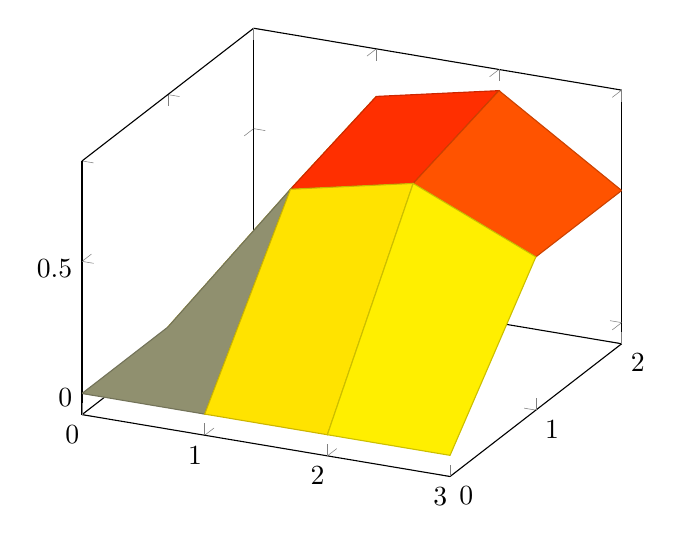
\begin{tikzpicture}
	\begin{axis}
		% this yields a 3x4 matrix:
		\addplot3[surf] coordinates {
			(0,0,0) (1,0,0)   (2,0,0)   (3,0,0)

			(0,1,0) (1,1,0.6) (2,1,0.7) (3,1,0.5)

			(0,2,0) (1,2,0.7) (2,2,0.8) (3,2,0.5)
		};
	\end{axis}
\end{tikzpicture}
\end{codeexample}
	\noindent Here, \verbpdfref{\addplot3} reads a matrix with three rows and four columns. The |empty line|s separate one row from the following.

	As for the two--dimensional |plot coordinates|, it is possible to provide (constant) mathematical expressions inside of single coordinates. The syntax |(|\meta{x}|,|\meta{y}|,|\meta{z}|) |\oarg{meta} can be used just as for two dimensional |plot coordinates| to provide explicit color data; error bars are also supported.
\end{addplot3operation}

\begin{addplot3operation}[]{file}{\marg{name}}
	The \verbpdfref{\addplot3 file} input method is the same as \verbpdfref{\addplot file} -- it only expects one more coordinate.
	Thus, the input file contains $x_i$ in the first column, $y_i$ in the second column and $z_i$ in the third. 
	
	A further column is read after $z_i$ if |point meta=explicit| has been requested, see the documentation of \verbpdfref{\addplot file} on page~\pageref{pgfplots:addplot:file} for details.
	
	As for \verbpdfref{\addplot3 coordinates}, an |empty line| in the file marks the end of one matrix row.
\begin{codeexample}[]
\begin{tikzpicture}
	\begin{axis}
		% We have `plotdata/first3d.dat' with
		%---------
		% 0 0 0.8
		% 1 0 0.56
		% 2 0 0.5
		% 3 0 0.75
		%
		% 0 1 0.6
		% 1 1 0.3
		% 2 1 0.21
		% 3 1 0.3
		%
		% 0 2 0.68
		% 1 2 0.22
		% 2 2 0.25
		% 3 2 0.4
		%
		% 0 3 0.7
		% 1 3 0.5
		% 2 3 0.58
		% 3 3 0.9
		% -> yields a 4x4 matrix:
		\addplot3[surf] file {plotdata/first3d.dat};
	\end{axis}
\end{tikzpicture}
\end{codeexample}

	For matrix data in files, it is important to specify the ordering in which the matrix entries have been written. The default configuration is |mesh/ordering=x varies|, so you need to change it to |mesh/ordering=y varies| in case you have columnwise ordering.
\end{addplot3operation}

\begin{addplot3operation}[]{table}{\oarg{column selection}\marg{file}}
	The \verbpdfref{\addplot3 table} input works in the same way as its two dimensional counterpart \verbpdfref{\addplot table}. It only expects a column for the $z$ coordinates. Furthermore, it interprets empty input lines as end--of--row (more generally, end--of--scanline) markers, just as for |plot file|. The remark above about the |mesh/ordering| applies here as well.
\end{addplot3operation}

\begin{pgfplotskeylist}{mesh/rows=\marg{integer},mesh/cols=\marg{integer}}
	For visualization of mesh or surface plots which need some sort of matrix input, the dimensions of the input matrix need to be known in order to visualize the plots correctly. The matrix structure may be known from end--of--row marks (|empty line|s as general end--of--scanline markers in the input stream) as has been described above.

	If the matrix structure is not yet known, it is necessary to provide at least one of |mesh/rows| or |mesh/cols| where |mesh/rows| indicates the number of samples for $y$ coordinates whereas |mesh/cols| is the number of samples used for $x$ coordinates (see also |mesh/ordering|). 

	Thus, the following example is also a valid method to define an input matrix.
\begin{codeexample}[]
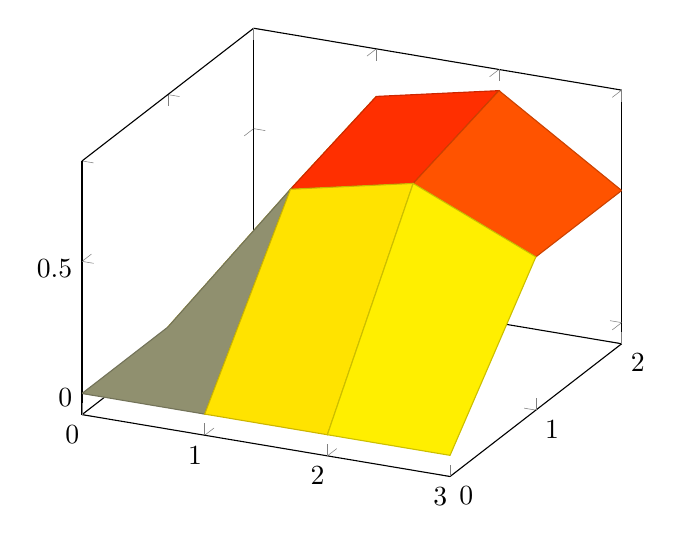
\begin{tikzpicture}
	\begin{axis}
		% this yields also a 3x4 matrix:
		\addplot3[surf,mesh/rows=3] coordinates {
			(0,0,0) (1,0,0)   (2,0,0)   (3,0,0)
			(0,1,0) (1,1,0.6) (2,1,0.7) (3,1,0.5)
			(0,2,0) (1,2,0.7) (2,2,0.8) (3,2,0.5)
		};
	\end{axis}
\end{tikzpicture}
\end{codeexample}

	It is enough to supply one of |mesh/rows| or |mesh/cols| -- the missing value will be determined automatically.
	
	If you provide one of |mesh/rows| or |mesh/cols|, any end--of--row marker seen inside of input files or coordinate streams will be ignored.

\end{pgfplotskeylist}

\begin{pgfplotskeylist}{mesh/scanline verbose=\mchoice{true,false} (initially false)}
	Provides debug messages in the \LaTeX\ output about end--of--scanline markers.

	The message will tell whether end--of--scanlines have been found and if they are the same.
\end{pgfplotskeylist}

\begin{pgfplotskey}{mesh/ordering=\mchoice{x varies,y varies,rowwise,colwise} (initially x varies)}
	Allows to configure the sequence in which matrices (meshes) are read from \verbpdfref{\addplot3 coordinates}, \verbpdfref{\addplot3 file} or \verbpdfref{\addplot3 table}.

	Here, \declaretext{x varies} means a sequence of points where $n$=|mesh/cols| successive points have the $y$ coordinate fixed. This is intuitive when you write down a function because $x$ is horizontal and $y$ vertical. Note that in matrix terminology, $x$ refers to \emph{column indices} whereas $y$ refers to \emph{row indices}. Thus, |x varies| is equivalent to \declaretext{rowwise} ordering in this sense. This is the initial configuration.
	
\long\def\temporarytest{\noexpand\par}
\begin{codeexample}[newline=\temporarytest]
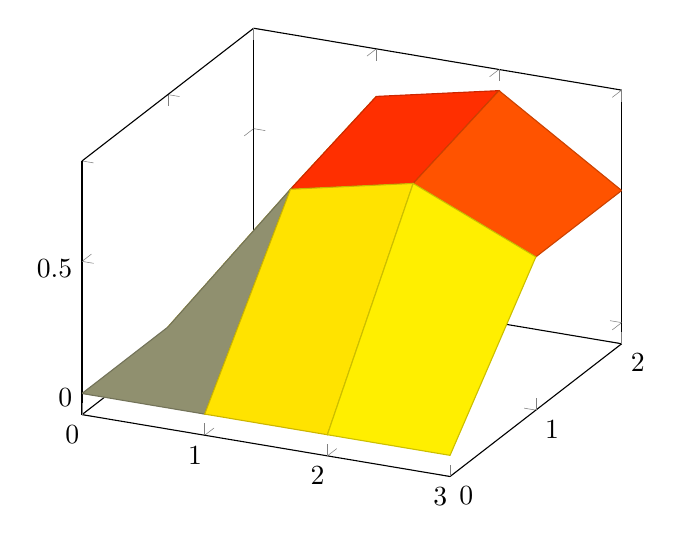
\begin{tikzpicture}
\begin{axis}[mesh/ordering=x varies]
	% this yields a 3x4 matrix in `x varies'
	% ordering:
	\addplot3[surf] coordinates {
		(0,0,0) (1,0,0)   (2,0,0)   (3,0,0)

		(0,1,0) (1,1,0.6) (2,1,0.7) (3,1,0.5)

		(0,2,0) (1,2,0.7) (2,2,0.8) (3,2,0.5)
	};
\end{axis}
\end{tikzpicture}
\end{codeexample}
	\noindent Note that |mesh/ordering| is mandatory, even though the size of the matrix can be provided in different ways. The example above uses |empty line|s to mark scanlines. One could also say |mesh/rows=3| and omit the |empty line|s.

	Consequently, |mesh/ordering=|\declaretext{y varies} provides points such that successive $m$=|mesh/rows| points form a column, i.e. the $x$ coordinate is fixed and the $y$ coordinate changes. In this sense, |y varies| is equivalent to \declaretext{colwise} ordering, it is actually a matrix transposition.
\long\def\temporarytest{\noexpand\par}
\begin{codeexample}[newline=\temporarytest]
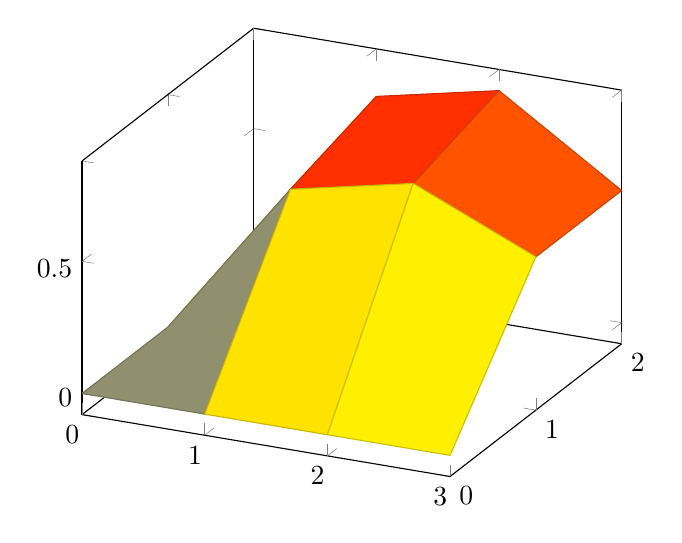
\begin{tikzpicture}
\begin{axis}[mesh/ordering=y varies]
	% this yields a 3x4 matrix in colwise ordering:
	\addplot3[surf] coordinates {
		(0,0,0) (0,1,0)   (0,2,0)

		(1,0,0) (1,1,0.6) (1,2,0.7)

		(2,0,0) (2,1,0.7) (2,2,0.8)

		(3,0,0) (3,1,0.5) (3,2,0.5)
	};
\end{axis}
\end{tikzpicture}
\end{codeexample}
	Again, note the subtle difference to the common matrix indexing where a column has the second index fixed. \PGFPlots\ refers to the way one would write down a function on a sheet of paper (this is consistent with how Matlab (\textregistered) displays discrete functions with matrices).

\end{pgfplotskey}

\begin{addplot3operation}[]{\marg{math expression}}{}
\label{cmd:addplot3:expr}
	\pgfmanualpdflabel{\textbackslash addplot3 expression}{}%
	Expression plotting also works in the same way as for two dimensional plots. Now, however, a two dimensional mesh is sampled instead of a single line, which may depend on |x| and |y|.

	The method \verbpdfref{\addplot3} \marg{math expr} visualizes the function $f(x,y) = $\meta{math expr} where $ f \colon [x_1,x_2] \times [y_1,y_2] \to \R$. The interval $[x_1,x_2]$ is determined using the |domain| key, for example using |domain=0:1|. The interval $[y_1,y_2]$ is determined using the |y domain| key. If |y domain| is empty, $[y_1,y_2] = [x_1,x_2]$ will be assumed. If |y domain=0:0| (or any other interval of length zero), it is assumed that the plot does not depend on |y| (thus, it is a line plot).

	The number of samples in $x$ direction is set using the |samples| key. The number of samples in $y$ direction is set using the |samples y| key. If |samples y| is not set, the same value as for $x$ is used. If |samples y|$\,\le 1$, it is assumed that the plot does not depend on |y| (meaning it is a line plot).

\pgfplotsexpensiveexample
\begin{codeexample}[]
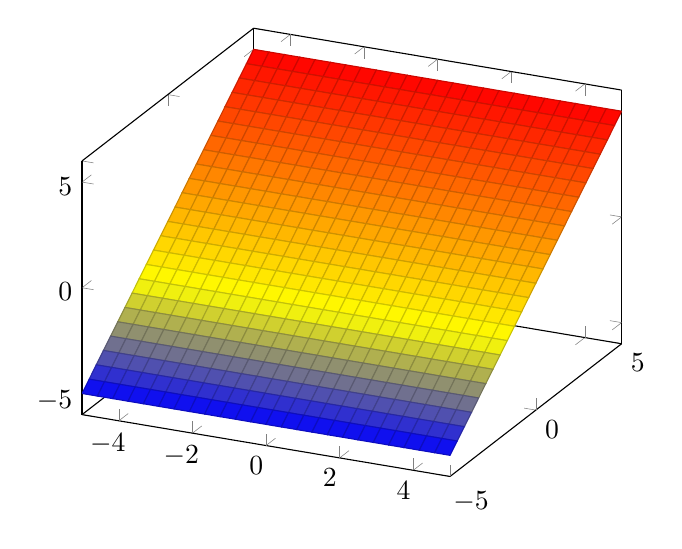
\begin{tikzpicture}
	\begin{axis}
		\addplot3[surf] {y};
	\end{axis}
\end{tikzpicture}
\end{codeexample}

\pgfplotsexpensiveexample
\begin{codeexample}[]
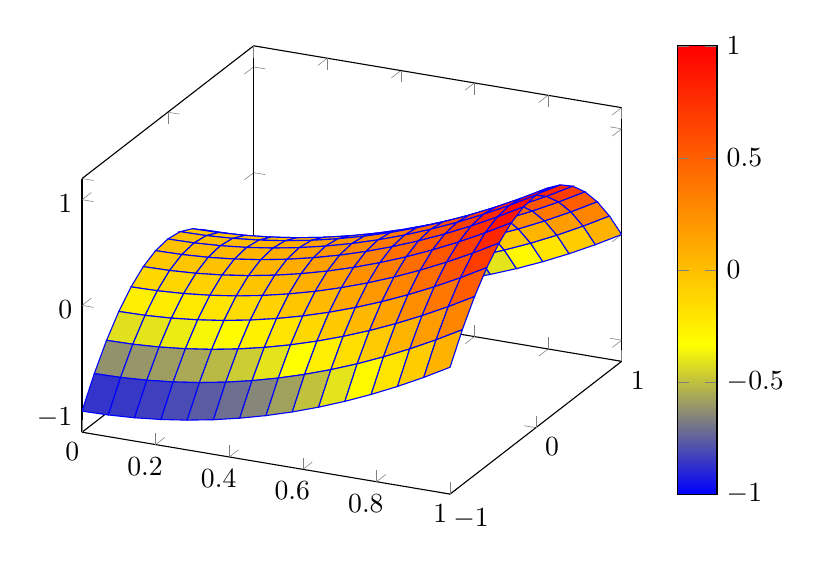
\begin{tikzpicture}
	\begin{axis}[colorbar]
		\addplot3
			[surf,faceted color=blue,
			 samples=15,
			 domain=0:1,y domain=-1:1]
			{x^2 - y^2};
	\end{axis}
\end{tikzpicture}
\end{codeexample}

	Expression plotting sets |mesh/rows| and |mesh/cols| automatically; these settings don't have any effect for expression plotting.
\end{addplot3operation}

\begin{addplot3operation}[]{expression}{\marg{math expression}}
	The syntax

	\verbpdfref{\addplot3} \marg{math expression}|;|

	as short-hand equivalent for

	\verbpdfref{\addplot3 expression} \marg{math expression}|;|
\end{addplot3operation}

\begin{addplot3operation}[]{(\meta{$x$ expression},\meta{$y$ expression},\meta{$z$ expression})}{}
	A variant of \verbpdfref{\addplot3 expression} which allows to provide different coordinate expressions for the $x$, $y$ and $z$ coordinates. This can be used to generate parametrized plots.

	Please note that |\addplot3 (x,y,x^2)| is equivalent to |\addplot3 expression {x^2}|.

	Note further that since the complete point expression is surrounded by round braces, round braces inside of \meta{$x$ expression}, \meta{$y$ expression} or \meta{$z$ expression} need to be treated specially. Surround the expressions (which contain round braces) with curly braces:

	|\addplot3 (|\marg{$x$ expr}|, |\marg{$y$ expr}|, |\marg{$z$ expr}|);|
\end{addplot3operation}

\subsubsection{Line Plots}

Three dimensional line plots are generated if the input source has no matrix structure. Line plots take the input coordinates and connect them in the order of appearance.

\begin{codeexample}[]
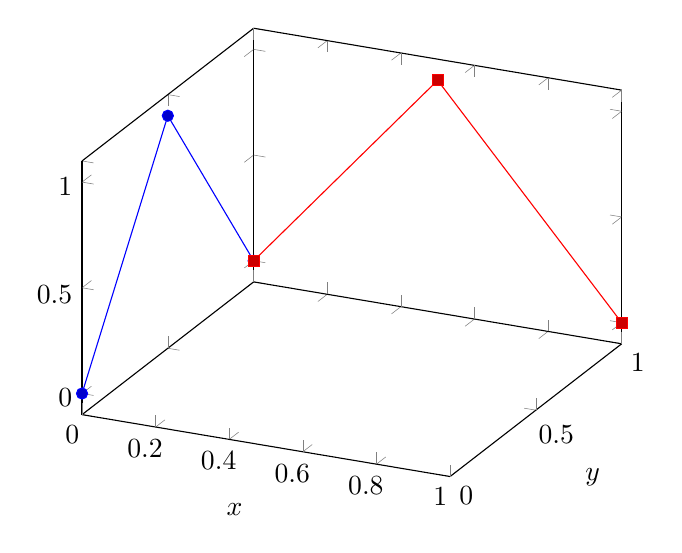
\begin{tikzpicture}
	\begin{axis}[xlabel=$x$,ylabel=$y$]
	\addplot3 coordinates {(0,0,0) (0,0.5,1) (0,1,0)};
	\addplot3 coordinates {(0,1,0) (0.5,1,1) (1,1,0)};
	\end{axis}
\end{tikzpicture}
\end{codeexample}
If there is no value for neither |mesh/rows| nor |mesh/cols| or if one of them is |1|, \PGFPlots\ will draw a line plot. This is also the case if there is no end--of--scanline marker (|empty line|) in the input stream.

For \verbpdfref{\addplot3 expression}, this requires to set |samples y=0| to disable the generation of a mesh.
\begin{codeexample}[]
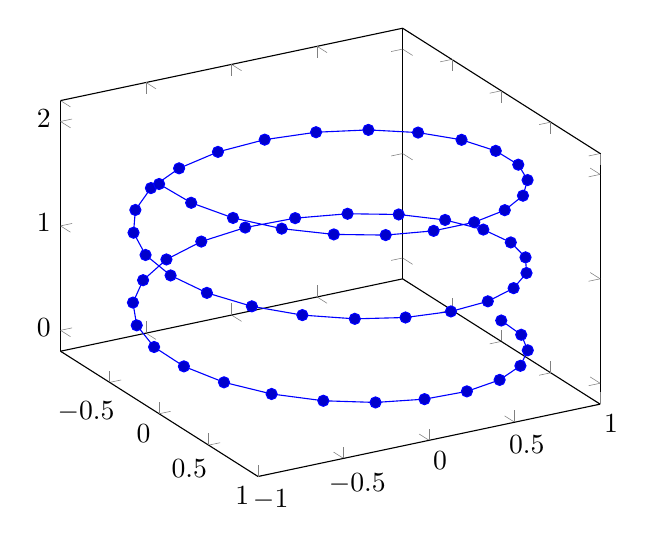
\begin{tikzpicture}
\begin{axis}[view={60}{30}]
\addplot3+[domain=0:5*pi,samples=60,samples y=0] 
	({sin(deg(x))},
	 {cos(deg(x))},
	 {2*x/(5*pi)});
\end{axis}
\end{tikzpicture}
\end{codeexample}
\noindent The example above is a parametric plot by expression, i.e.\ it has three distinct expressions for $x$, $y$, and $z$.

Line plots in three dimensions are also possible for data plots (tables). The most simple case is if you simply provide a series of three--dimensional coordinates which will be connected in the order of appearance:
\begin{codeexample}[]
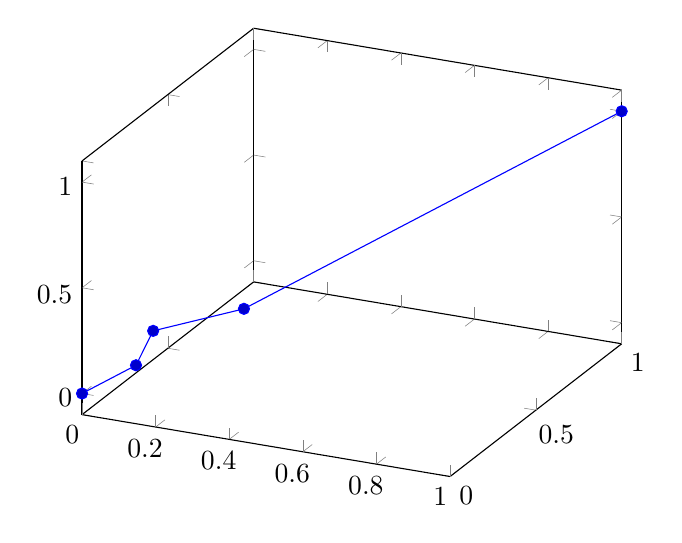
\begin{tikzpicture}
\begin{axis}
\addplot3 table {
	x   y   z
	0   0   0
	0.1 0.1 0.1
	0.1 0.2 0.2
	0.3 0.3 0.3
	1   1   1
	};
\end{axis}
\end{tikzpicture}
\end{codeexample}
\noindent Note that this plot implicitly has |mesh/rows=1| because it has no end--of--scanline markers (|empty line|s). If in doubt, you can set |mesh/rows=1| explicitly to tell \PGFPlots\ that you have one--dimensional data (and not a matrix).

Line plots from data files are also possible if the data files only contains two coordinates -- and the third should be provided somehow. In this case, the |table/x expr| feature comes into play: it allows to combine data plots and math expressions:
\begin{codeexample}[]
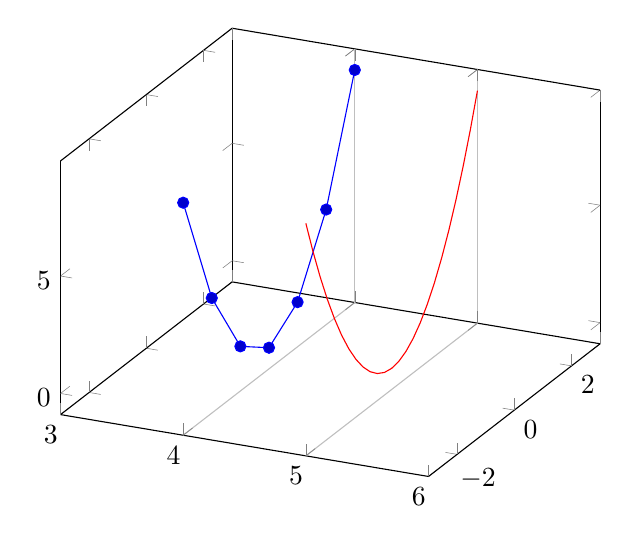
\begin{tikzpicture}
\begin{axis}[
	xmin=3,xmax=6,
	extra x ticks={4,5}, 
	extra x tick style={xticklabel=\empty,grid=major}
]
\addplot3 table[x expr=4,y=a,z=b] {
a  b
-3 9
-2 4
-1 1
0  0
1  1
2  4
3  9
};
\addplot3[red,domain=-3:3,samples y=0] (5,x,x^2);
\end{axis}
\end{tikzpicture}
\end{codeexample}
\noindent Here, we have two plots in one axis: one data plot from a data table with just two coordinates and one parametric plot. Both denote the same two functions. For the data plot, |x expr=4| assigns the $x$ coordinate, and |y=a,z=b| define how the input columns map to coordinates. Again, the plot implicitly uses |mesh/rows=1| since there is no end--of--scanline marker. The second plot does the same with the short--handed notation |(5,x,x^2)|. It only samples one--dimensional data due to |samples y=0|. Finally, |extra x ticks| configures two additional ticks for the $x$~axis; this is used to display grid lines for these specific ticks. The |xticklabel=\empty| argument avoids overprinted $x$~tick labels at positions $x\in\{4,5\}$.


Three dimensional line plots will usually employ lines to connect points (i.e.\ the initial |sharp plot| handler of \Tikz). The |smooth| method of \Tikz\ might also prove be an option. Note that no piecewise constant plot, comb or bar plot handler is supported for three dimensional axes.

\subsubsection{Scatter Plots}

Three dimensional scatter plots have the same interface as for two dimensional scatter plots, so all examples of Section~\ref{sec:pgfplots:scatter:2d} can be used for the three dimensional case as well. 
The key features are to use |only marks| and/or |scatter| as plot styles. 

We provide some more examples which are specific for the three dimensional case.

Our first example uses |only marks| to place the current plot |mark| at each input position:
\pgfplotsexpensiveexample
\begin{codeexample}[]
\begin{tikzpicture}
	\begin{axis}[
		xlabel=$x$,
		ylabel=$y$,
		zlabel={$f(x,y) = x\cdot y$},
		title=A Scatter Plot Example]
	% `pgfplotsexample4_grid.dat' contains a
	% large sequence of input points of the form
	% x_0   x_1     f(x)    
	% 0     0       0       
	% 0     0.03125 0       
	% 0     0.0625  0       
	% 0     0.09375 0       
	% 0     0.125   0       
	% 0     0.15625 0       
	\addplot3+[only marks] table
		{plotdata/pgfplotsexample4_grid.dat};
	\end{axis}
\end{tikzpicture}
\end{codeexample}

If we add the key |scatter|, the plot mark will also use the colors of the current |colormap|:
\pgfplotsexpensiveexample
\begin{codeexample}[]
\begin{tikzpicture}
	\begin{axis}[
		xlabel=$x$,
		ylabel=$y$,
		zlabel={$f(x,y) = x\cdot y$},
		title=A Scatter Plot Example]
	\addplot3+[only marks,scatter] table 
		{plotdata/pgfplotsexample4_grid.dat};
	\end{axis}
\end{tikzpicture}
\end{codeexample}

A more sophisticated example is to draw the approximated function as a |surf| plot (which requires matrix data) and the underlying grid (which is |scatter|ed data) somewhere into the same axis. We choose to place the $(x,y)$ grid points at $z=1.4$. Furthermore, we want the grid points to be colored according to the value of column |f(x)| in the input table:
\pgfplotsexpensiveexample
\begin{codeexample}[]
\begin{tikzpicture}
	\begin{axis}[
		3d box,
		zmax=1.4,
		colorbar,
		xlabel=$x$,
		ylabel=$y$,
		zlabel={$f(x,y) = x\cdot y$},
		title={Using Coordinate Filters to fix $z=1.4$}]
	% `pgfplotsexample4.dat' contains similar data as in 
	% `pgfplotsexample4_grid.dat', but it uses a uniform
	% matrix structure (same number of points in every scanline).
	% See examples above for extracts.
	\addplot3[surf,mesh/ordering=y varies] 
		table {plotdata/pgfplotsexample4.dat};
	\addplot3[scatter,scatter src=\thisrow{f(x)},only marks, z filter/.code={\def\pgfmathresult{1.4}}] 
		table {plotdata/pgfplotsexample4_grid.dat};
	\end{axis}
\end{tikzpicture}
\end{codeexample}
\noindent We used |z filter| to fix the $z$ coordinate to $1.4$. We could also have used the |table/z expr=1.4| feature
\begin{codeexample}[code only]
	\addplot3[scatter,scatter src=\thisrow{f(x)},only marks] 
		table[z expr=1.4] {plotdata/pgfplotsexample4_grid.dat};
\end{codeexample}
\noindent to get exactly the same effect. Choose whatever you like best. The |z filter| works for every coordinate input routine, the |z expr| feature is only available for |plot table|.


The following example uses |mark=cube*| and |z buffer=sort| to place boxes at each input coordinate. The color for each box is determined by |point meta={x+y+3}|. The remaining keys are just for pretty printing.
\pgfplotsexpensiveexample
\begin{codeexample}[]
\begin{tikzpicture}
\begin{axis}[
	view={120}{40},
	width=220pt,
	height=220pt,
	grid=major,
	z buffer=sort,
	xmin=-1,xmax=9,
	ymin=-1,ymax=9,
	zmin=-1,zmax=9,
	enlargelimits=upper,
	xtick={-1,1,...,19},
	ytick={-1,1,...,19},
	ztick={-1,1,...,19},
	xlabel={$l_1$},
	ylabel={$l_2$},
	zlabel={$l_3$},
	point meta={x+y+z+3},
	colormap={summap}{
		color=(black); color=(blue); 
		color=(black); color=(white) 
		color=(orange) color=(violet) 
		color=(red)
	},
	scatter/use mapped color={
		draw=mapped color,fill=mapped color!70},
	]
	% `pgfplots_scatter4.dat' contains a large sequence of
	% the form
	% l_0   l_1     l_2     
	% 1     6       -1      
	% -1    -1      -1      
	% 0     -1      -1      
	% -1    0       -1      
	% -1    -1      0       
	% 1     -1      -1      
	% 0     0       -1      
	% 0     -1      0       
	\addplot3[only marks,scatter,mark=cube*,mark size=7] 
		table {plotdata/pgfplots_scatterdata4.dat};

\end{axis}
\end{tikzpicture}
\end{codeexample}


\subsubsection{Mesh Plots}
\label{sec:2d:mesh}
\begin{plottype}[/pgfplots]{mesh}
	A mesh plot uses different colors for each mesh segment. The color is determined using a ``color coordinate'' which is also called ``meta data'' throughout this document. It is the same data which is used for surface and scatter plots as well, see Section~\ref{pgfplots:pointmeta}. In the initial configuration, the ``color coordinate'' is the $z$ axis (or the $y$ axis for two dimensional plots). This color coordinate is mapped linearly into the current color map to determine the color for each mesh segment. Thus, if the smallest occurring color data is, say, $-1$ and the largest is $42$, points with color data $-1$ will get the color at the lower end of the color map and points with color data $42$ the color of the upper end of the color map.

\pgfplotsexpensiveexample
\begin{codeexample}[]
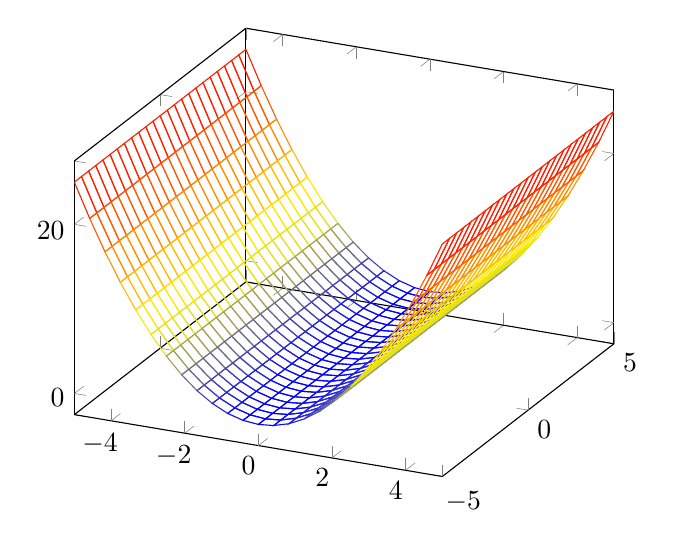
\begin{tikzpicture}
	\begin{axis}
		\addplot3[mesh] {x^2};
	\end{axis}
\end{tikzpicture}
\end{codeexample}

	A mesh plot can be combined with markers or with the |scatter| key which also draws markers in different colors.

\pgfplotsexpensiveexample
\begin{codeexample}[]
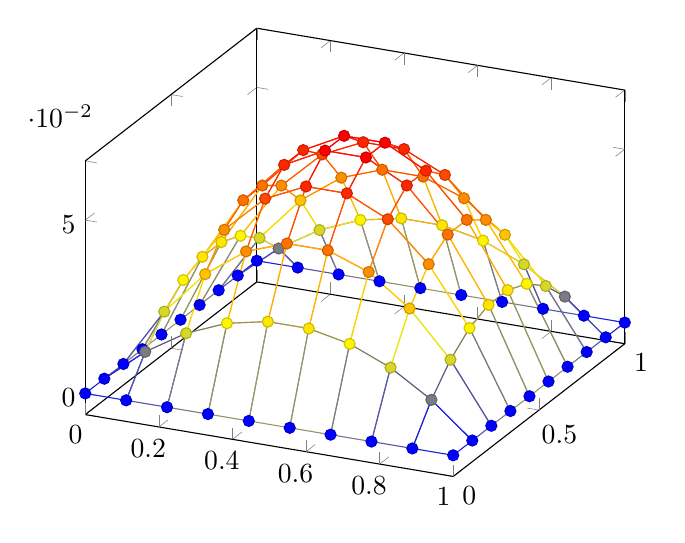
\begin{tikzpicture}
	\begin{axis}
	\addplot3+[mesh,scatter,samples=10,domain=0:1] 
		{x*(1-x)*y*(1-y)};
	\end{axis}
\end{tikzpicture}
\end{codeexample}

\pgfplotsexpensiveexample
\begin{codeexample}[]
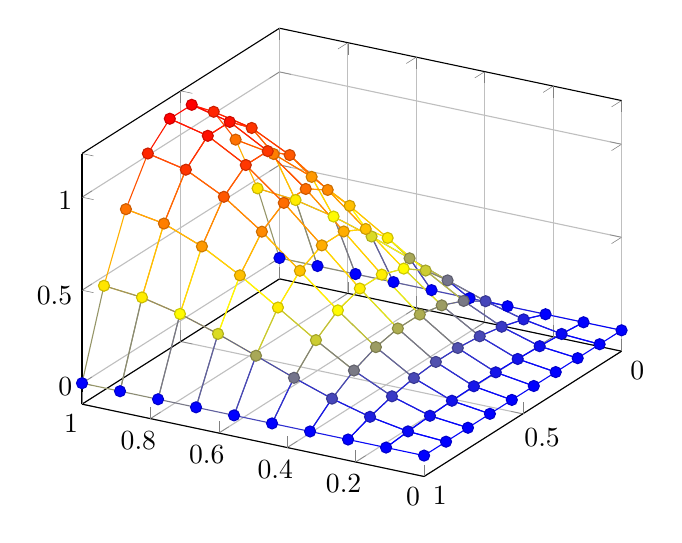
\begin{tikzpicture}
	\begin{axis}[grid=major,view={210}{30}]
	\addplot3+[mesh,scatter,samples=10,domain=0:1] 
		{5*x*sin(2*deg(x)) * y*(1-y)};
	\end{axis}
\end{tikzpicture}
\end{codeexample}

	Occasionally, one may want to hide the background mesh segments. This can be realized using the |surf| plot handler (see below) and a specific fill color:
\pgfplotsexpensiveexample
\begin{codeexample}[]
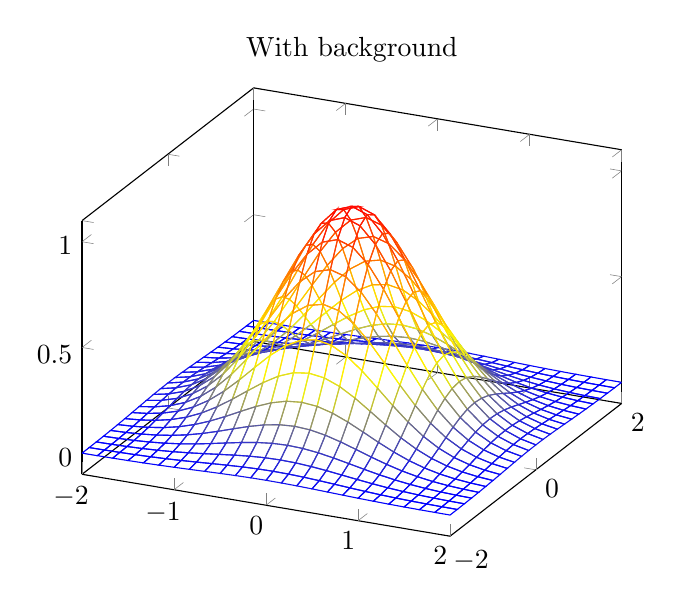
\begin{tikzpicture}
	\begin{axis}[title=With background]
	\addplot3[mesh,domain=-2:2] {exp(-x^2-y^2)};	
	\end{axis}
\end{tikzpicture}
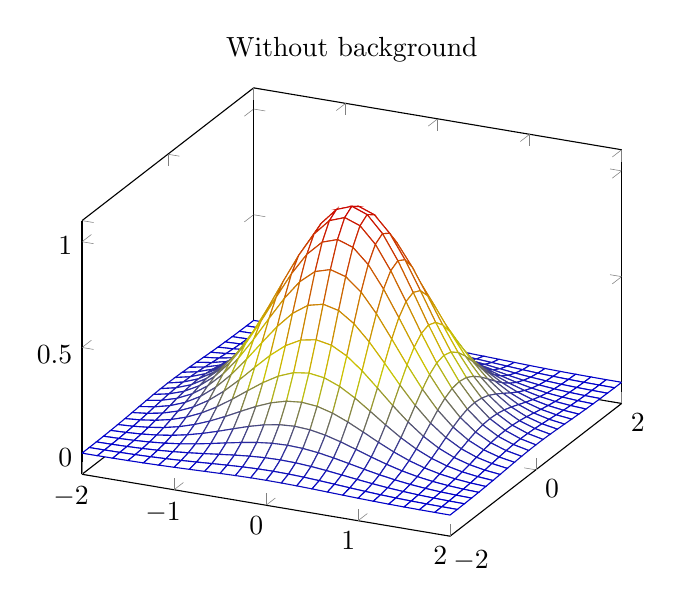
\begin{tikzpicture}
	\begin{axis}[title=Without background]
	\addplot3[surf,fill=white,domain=-2:2] {exp(-x^2-y^2)};	
	\end{axis}
\end{tikzpicture}
\end{codeexample}
	The fill color needs to be provided explicitly.

	\paragraph{Details:}
	\begin{itemize}
		\item 
	A mesh plot uses the same implementation as |shader=flat| to get one color for each single segment. Thus, if |shader=flat mean|, the color for a segment is determined using the \emph{mean} of the color data of adjacent vertices. If |shader=flat corner|, the color of a segment is the color of \emph{one} adjacent vertex.
		\item As soon as |mesh| is activated, |color=mapped color| is installed. This is \emph{necessary} unless one needs a different color -- but |mapped color| is the only color which reflects the color data.

		It is possible to use a different color using the |color=|\meta{color name} as for any other plot.

		\item It is easily possible to add |mark=|\meta{marker name} to mesh plots, |scatter| is also possible. Scatter plots will use the same color data as for the mesh.
	\end{itemize}

\pgfplotsexpensiveexample
\begin{codeexample}[]
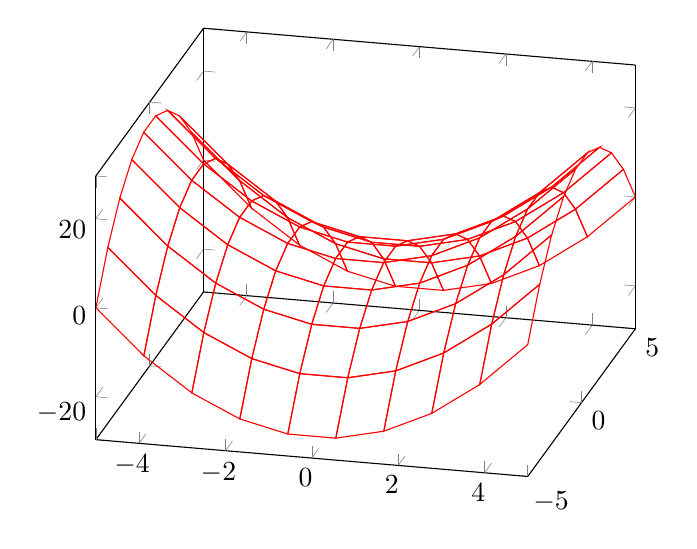
\begin{tikzpicture}
	\begin{axis}[view/az=14]
	\addplot3[mesh,draw=red,samples=10] {x^2-y^2};	
	\end{axis}
\end{tikzpicture}
\end{codeexample}
	
	Mesh plots use the |mesh legend| style to typeset legend images.
\end{plottype}

\begin{pgfplotskey}{mesh/check=\mchoice{false,warning,error} (initially error)}
	Allows to configure whether an error is generated if |mesh/rows| $\times$ |mesh/cols| does not equal the total number of coordinates.

	If you know exactly what you are doing, it may be useful to disable the check. If you are unsure, it is best to leave the initial setting.
\end{pgfplotskey}

\begin{pgfplotskey}{z buffer=\mchoice{default,none,auto,sort,reverse x seq,reverse y seq,reverse xy seq} (initially default)}
	This key allows to choose between different $z$ buffering strategies. A $z$ buffer determines which parts of an image should be drawn in front of other parts. Since both, the graphics packages \PGF\ and the final document format |.pdf| are inherently two dimensional, this work has to be done in \TeX. Currently, several (fast) heuristics can be used which work reasonably well for simple mesh- and surface plots. Furthermore, there is a (time consuming) sorting method which also works if the fast heuristics fails.

	The $z$ buffering algorithms of \PGFPlots\ apply only to a single |\addplot| command. Different |\addplot| commands will be drawn on top of each other, in the order of appearance.

	The choice \declaretext{default} checks if we are currently working with a mesh or surface plot and uses |auto| in this case. If not, it sets |z buffer=none|.

	The choice \declaretext{none} disables $z$ buffering. This is also the case for two dimensional axes which don't need $z$ buffering.

	The choice \declaretext{auto} is the initial value for any mesh or surface plot: it uses a very fast heuristics to decide how to realize $z$ buffering for mesh and surface plots. The idea is to reverse either the sequence of all $x$ coordinates, or those of all $y$ coordinates, or both. For regular meshes, this suffices to provide $z$ buffering. In other words: the choice |auto| will use one of the three reverse strategies |reverse |*| seq| (or none at all). The choice |auto|, applied to |patch| plots, uses |z buffer=sort| since |patch| plots have no matrix structure.

	The choice \declaretext{sort} can be used for scatter, line, mesh, surface and patch plots. It sorts according to the depth of each point (or mesh segment). Sorting in \TeX\ uses a slow algorithm and may require a lot of memory (although it has the expected runtime asymptotics $\mathcal O(N \log N)$). The depth of a mesh segment is just \emph{one} number, currently determined as \emph{mean} over the vertex depths. Since |z buffer=sort| is actually just a more intelligent way of drawing mesh segments on top of each other, it may still fail. Failure can occur if mesh segments are large and overlap at different parts of the segment (see Wikipedia ``Painter's algorithm''). If you experience problems of this sort, consider reducing the mesh width (the mesh element size) such that they can be sorted independently (for example automatically using |patch refines=2|, see the |patchplots| library).

	The remaining choices apply only to mesh/surface plots (i.e.\ for matrix data) and do nothing more then their name indicates: they reverse the coordinate sequences of the input matrix (using quasi linear runtime). They should only be used in conjunction by |z buffer=auto|.
\end{pgfplotskey}

\subsubsection{Surface Plots}
\label{sec:pgfplots:surfplots}
\begin{plottype}[/pgfplots]{surf}
	A surface plot visualizes a two dimensional, single patch using different fill colors for each patch segment. Each patch segment is a (pseudo) rectangle, that means input data is given in form of a data matrix as is discussed in the introductory section about three dimensional coordinates,~\ref{pgfplots:sec:threedim}.

\pgfplotsexpensiveexample
\begin{codeexample}[]
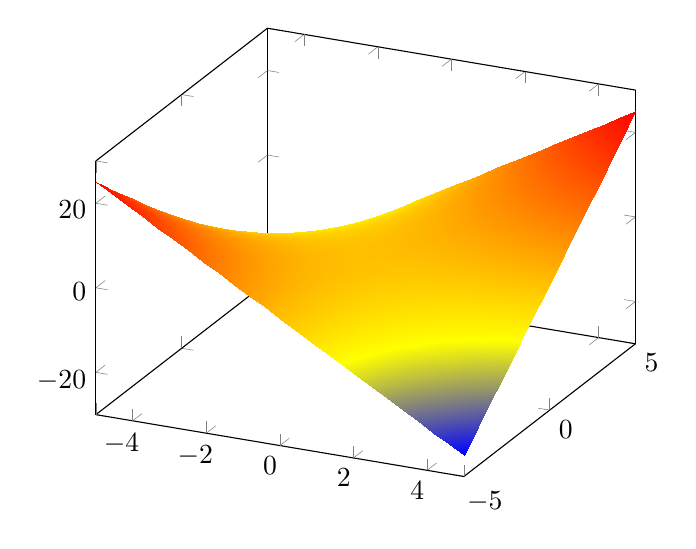
\begin{tikzpicture}
	\begin{axis}
		\addplot3[surf,shader=interp] {x*y};
	\end{axis}
\end{tikzpicture}
\end{codeexample}

	The simplest way to generate surface plots is to use the plot expression feature, but -- as discussed in Section~\ref{pgfplots:sec:threedim} -- other input methods like \verbpdfref{\addplot3 table} or \verbpdfref{\addplot3 coordinates} are also possible. 

	The appearance can be configured using |colormap|s, the value of the |shader|, |faceted color| keys and the current |color| and/or |draw|/|fill| color. As for |mesh| plots, the special |color=mapped color| is installed for the faces. The stroking color for faceted plots can be set with |faceted color| (see below for details).

\pgfplotsexpensiveexample
\begin{codeexample}[]
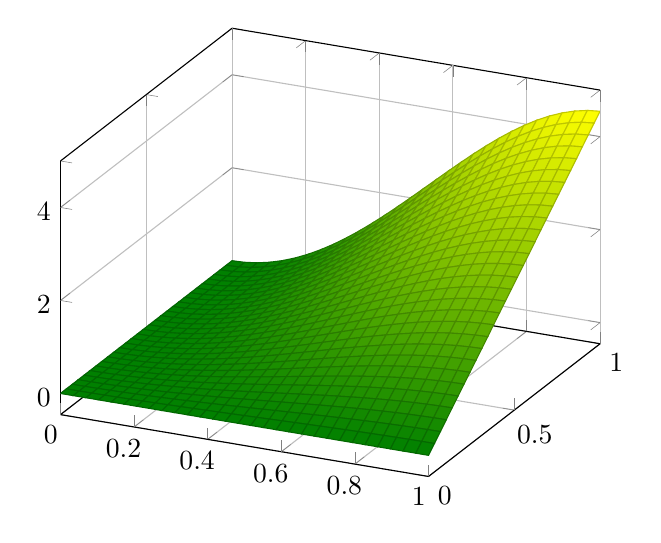
\begin{tikzpicture}
	\begin{axis}[
		grid=major,
		colormap/greenyellow]
	\addplot3[surf,samples=30,domain=0:1] 
		{5*x*sin(2*deg(x)) * y};
	\end{axis}
\end{tikzpicture}
\end{codeexample}

\pgfplotsexpensiveexample
\begin{codeexample}[]
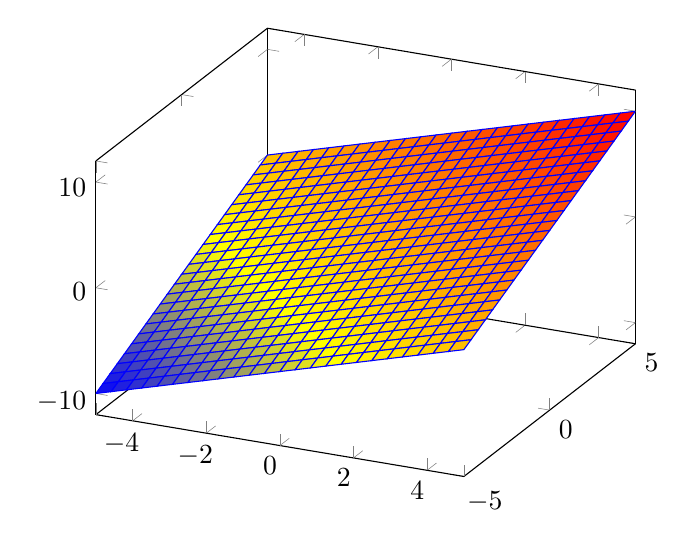
\begin{tikzpicture}
	\begin{axis}
		\addplot3[surf,faceted color=blue] {x+y};
	\end{axis}
\end{tikzpicture}
\end{codeexample}

\pgfplotsexpensiveexample
\begin{codeexample}[]
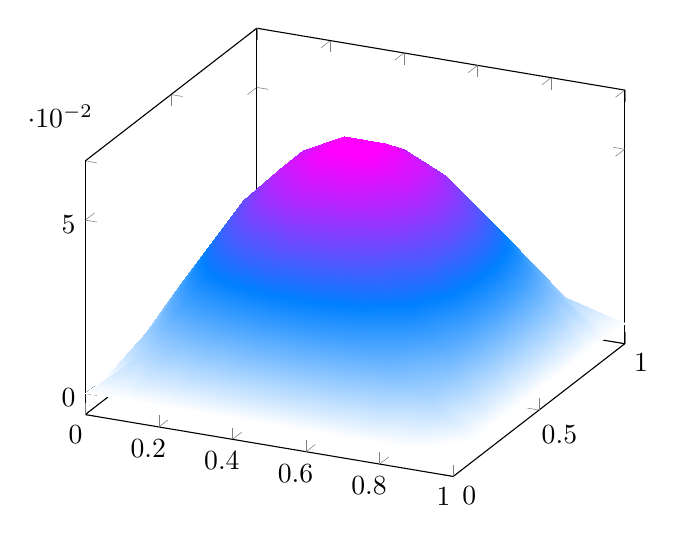
\begin{tikzpicture}
	\begin{axis}[colormap/cool]
	\addplot3[surf,samples=10,domain=0:1,
		shader=interp] 
		{x*(1-x)*y*(1-y)};
	\end{axis}
\end{tikzpicture}
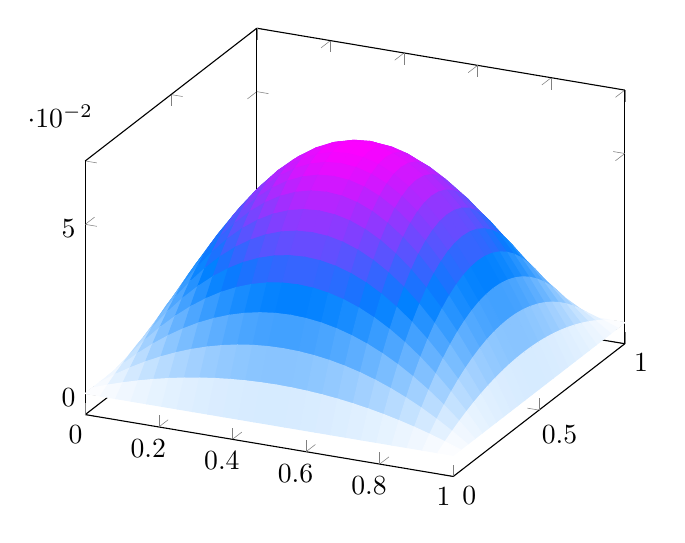
\begin{tikzpicture}
	\begin{axis}[colormap/cool]
	\addplot3[surf,samples=25,domain=0:1,
		shader=flat] 
		{x*(1-x)*y*(1-y)};
	\end{axis}
\end{tikzpicture}
\end{codeexample}

\pgfplotsexpensiveexample
\begin{codeexample}[]
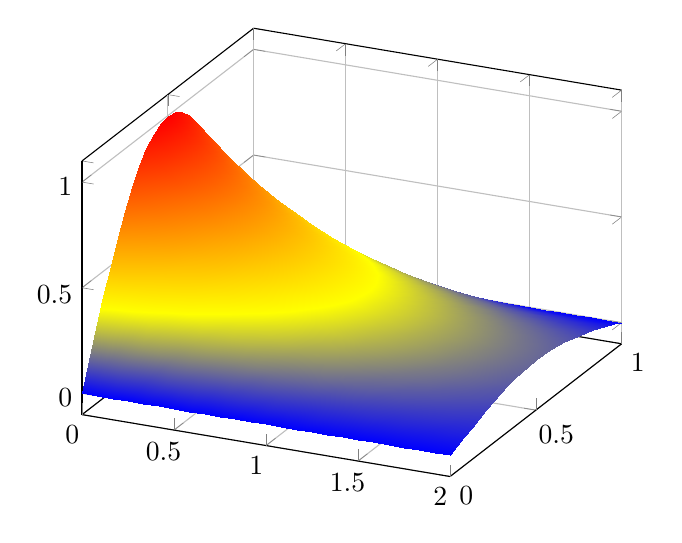
\begin{tikzpicture}
	\begin{axis}[grid=major]
		\addplot3[surf,shader=interp,
			samples=25,domain=0:2,y domain=0:1] 
			{exp(-x) * sin(pi*deg(y))};
	\end{axis}
\end{tikzpicture}
\end{codeexample}

\pgfplotsexpensiveexample
\begin{codeexample}[]
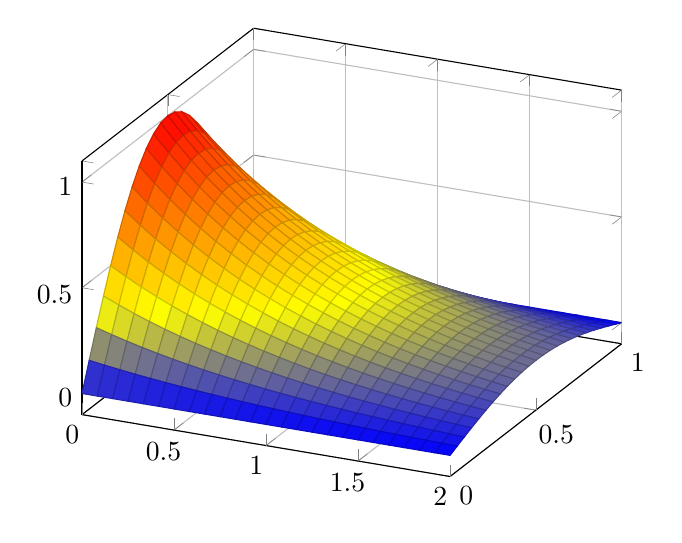
\begin{tikzpicture}
	\begin{axis}[grid=major]
		\addplot3[surf,shader=faceted,
			samples=25,domain=0:2,y domain=0:1] 
			{exp(-x) * sin(pi*deg(y))};
	\end{axis}
\end{tikzpicture}
\end{codeexample}

	Details about the shading algorithm are provided below in the documentation of |shader|.

	Surface plots use the |mesh legend| style to create legend images.
\end{plottype}

\begin{pgfplotskey}{shader=\mchoice{flat,interp,faceted,flat corner,flat mean,faceted interp} (initially faceted)}
	Configures the shader used for surface plots. The shader determines how the color data available at each single vertex is used to fill the surface patch.

	The simplest choice is to use one fill color for each segment, the choice \declareandlabel{flat}.

\pgfplotsexpensiveexample
\begin{codeexample}[]
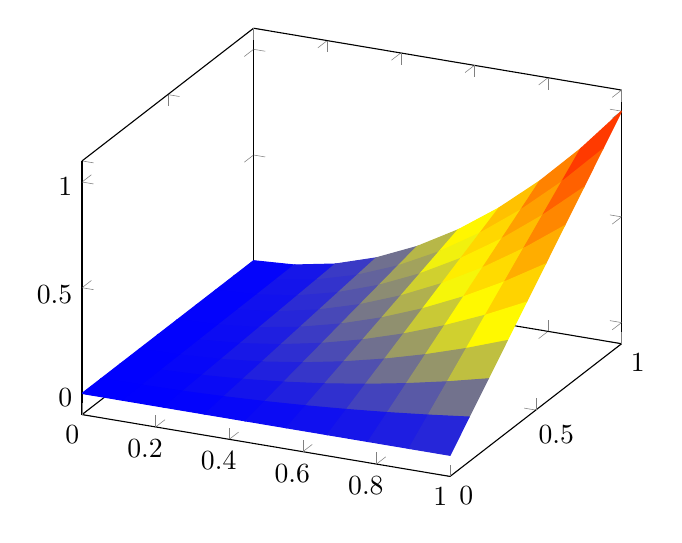
\begin{tikzpicture}
	\begin{axis}
	\addplot3[surf,shader=flat,
		samples=10,domain=0:1] 
		{x^2*y};
	\end{axis}
\end{tikzpicture}
\end{codeexample}

	\noindent There are (currently) two possibilities to determine the single color for every segment:
	\begin{description}
		\item[\declaretext{flat corner}] Uses the color data of one vertex to color the segment. It is not defined which vertex is used here\footnote{\PGFPlots\ just uses the last vertex encountered in its internal processings -- but after any $z$ buffer re-orderings.}.

		\item[\declaretext{flat mean}] Uses the mean of all four color data values as segment color. This is the initial value as it provides symmetric colors for symmetric functions.
	\end{description}
	The choice |flat| is actually the same as |flat mean|. Please note that |shader=flat mean| and |shader=flat corner| also influence mesh plots -- the choices determine the mesh segment color.

	Another choice is |shader=|\declareandlabel{interp} which uses Goraud shading (smooth linear interpolation of two triangles approximating rectangles) to fill the segments. 

\pgfplotsexpensiveexample
\begin{codeexample}[]
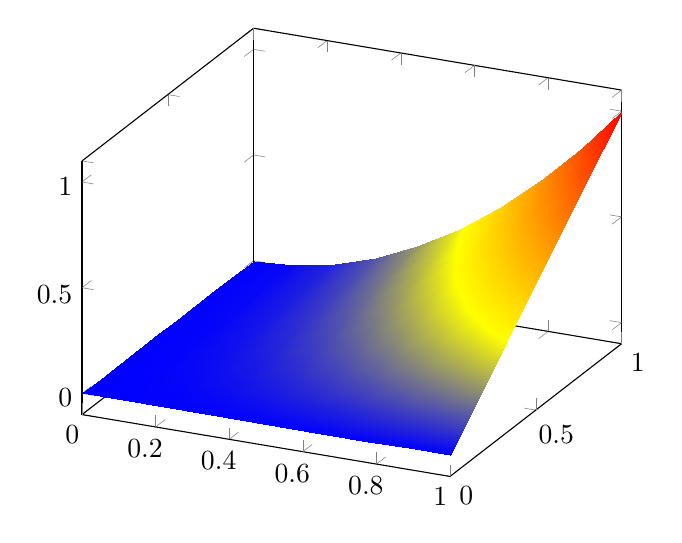
\begin{tikzpicture}
	\begin{axis}
	\addplot3[surf,shader=interp,
		samples=10,domain=0:1] 
		{x^2*y};
	\end{axis}
\end{tikzpicture}
\end{codeexample}

	The |shader=interp| employs a low--level shading implementation which is currently (only) available for the postscript driver \declaretext{pgfsys-dvips.def} and the |pdflatex| driver \declaretext{pgfsys-pdftex.def}. For other drivers, the choice |shader=interp| will result in a warning and is equivalent to |shader=flat mean|. See also below for detail remarks.
	
	Note that |shader=interp,patch type=bilinear| allows real bilinear interpolation, see the |patchplots| library.


	The choice |shader=|\declareandlabel{faceted} uses a constant fill color for every mesh segment (as for |flat|) and the value of the key |/pgfplots/faceted color| to draw the connecting mesh elements:
\pgfplotsexpensiveexample
\begin{codeexample}[]
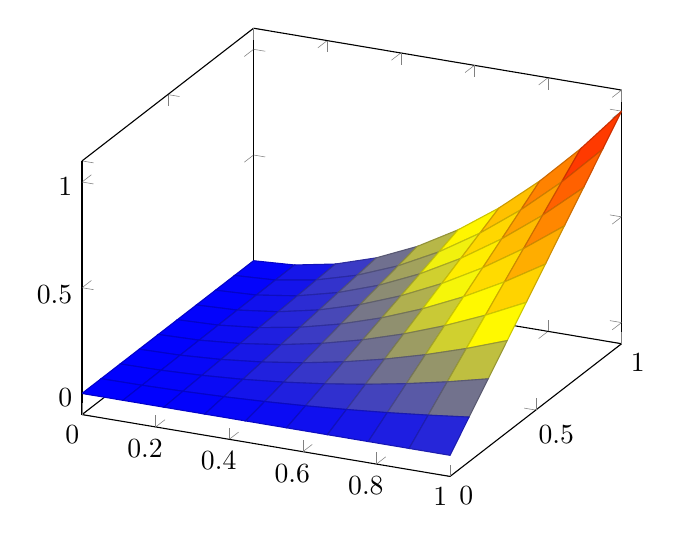
\begin{tikzpicture}
	\begin{axis}
	\addplot3[surf,shader=faceted,
		samples=10,domain=0:1] 
		{x^2*y};
	\end{axis}
\end{tikzpicture}
\end{codeexample}

	The last choice is |shader=|\declareandlabel{faceted interp}. As the name suggests, it is a mixture of |interp| and |faceted| in the sense that each element is shaded using linear triangle interpolation (see also the |patchplots| library for bilinear interpolation) in the same way as for |interp|, but additionally, the edges are colored in |faceted color|:
\pgfplotsexpensiveexample
\begin{codeexample}[]
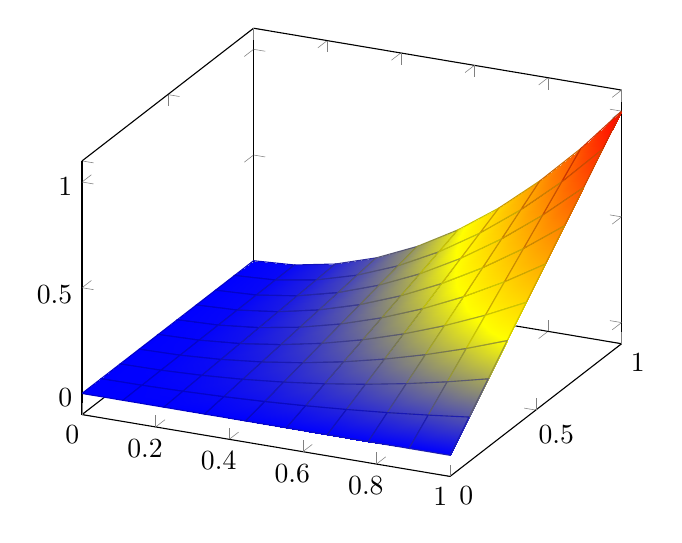
\begin{tikzpicture}
	\begin{axis}
	\addplot3[surf,shader=faceted interp,
		samples=10,domain=0:1] 
		{x^2*y};
	\end{axis}
\end{tikzpicture}
\end{codeexample}
	\noindent In principle, there is nothing wrong with the idea as such, and it looks quite good -- but it enlarges the resulting pdf document considerably and might take a long time to render. It works as follows: for every mesh element (either triangle for |patch| plots or rectangle for lattice plots), it creates a low level shading. It then fills the single mesh element with that shading, and strokes the edges with |faceted color|. The declaration of that many low level shadings is rather inefficient in terms of pdf objects (large output files) and might render slowly\footnote{My experience is as follows: Acrobat reader can efficiently render huge \texttt{interp} shadings. But it is very slow for \texttt{faceted interp} shadings. Linux viewers like xpdf are reasonably efficient for \texttt{interp} (at least with my bugfixes to libpoppler) and are also fast for \texttt{faceted interp} shadings.}. For orthogonal plots (like |view={0}{90}|), the effect of |faceted interp| can be gained with less cost if one uses two separate |\addplot| commands: one with |surf| and one with |mesh|. Handle this choice with care.

	\paragraph{Details:}
	\begin{itemize}
		\item All shaders support |z buffer=sort| (starting with version 1.4)
		\item The choice |shader=faceted| is the same as |shader=flat| -- except that it uses a special draw color.
		
		So, |shader=faceted| has the same effect as 
		
		|shader=flat,draw=\pgfkeysvalueof{/pgfplots/faceted color}|.

		\item The |flat| shader uses the current |draw| and |fill| colors. They are set with |color=mapped color| and can be overruled with |draw=|\meta{draw color} and |fill=|\meta{fill color}. The |mapped color| always contains the color of the color map. 

		\item You easily add |mark=|\meta{plot mark} to mesh and/or surface plots or even colored plot marks with |scatter|. The scatter plot feature will use the same color data as for the surface.

		But: Markers and surfaces do not share the same depth information. They are drawn on top of each other.

		
		\item Remarks on |shader=interp|:
			\begin{itemize}
				\item It uses the current color map in any case, ignoring |draw| and |fill|.
				\item For surface plots with lots of points, |shader=interp| produces smaller |pdf| documents, requires less compilation time in \TeX\ and requires less time to display in Acrobat Reader than |shader=flat|.

				\item The postscript driver \emph{truncates} coordinates to 24 bit -- which might result in a loss of precision (the truncation is not very intelligent). See the |surf shading/precision| key for details. To improve compatibility, this 24 bit truncation algorithm is enabled by default also for pdf documents.
				\item The choice |shader=interp| works well with either Acrobat Reader or recent versions of free viewers\footnote{The author of this package has submitted bugfixes to xpdf/libpoppler which should be part of the current stable versions of many viewers.}. However, some free viewers show colors incorrectly (like evince).  I hope this message will soon become outdated... if not, provide bug reports to the Linux community to communicate the need to improve support for Type 4 (|patch|) and Type 5 pdf (|surf|) and Type 7 (|patch| and elements of the |patchplots| library) shadings.
				\item The |interp| shader yields the same outcome as |faceted interp,faceted color=none|, although |faceted interp| requires much more ressources.
			\end{itemize}
	\end{itemize}

\pgfplotsexpensiveexample
\begin{codeexample}[]
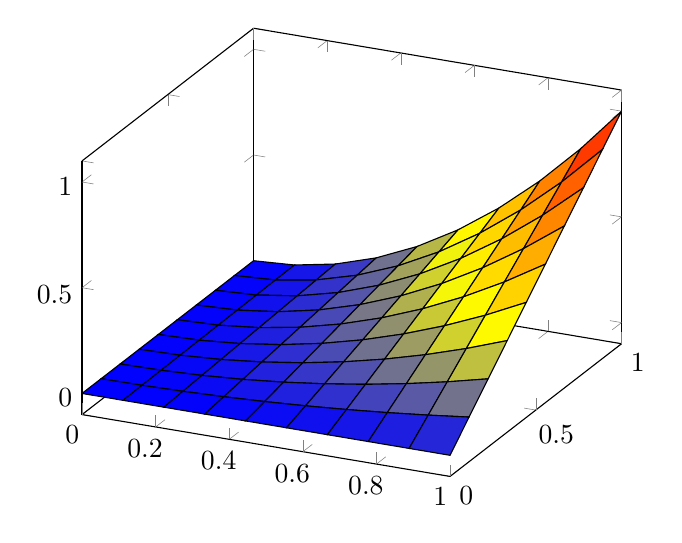
\begin{tikzpicture}
	\begin{axis}
	\addplot3[surf,shader=flat,
		draw=black,
		samples=10,domain=0:1] 
		{x^2*y};
	\end{axis}
\end{tikzpicture}
\end{codeexample}

\pgfplotsexpensiveexample
\begin{codeexample}[]
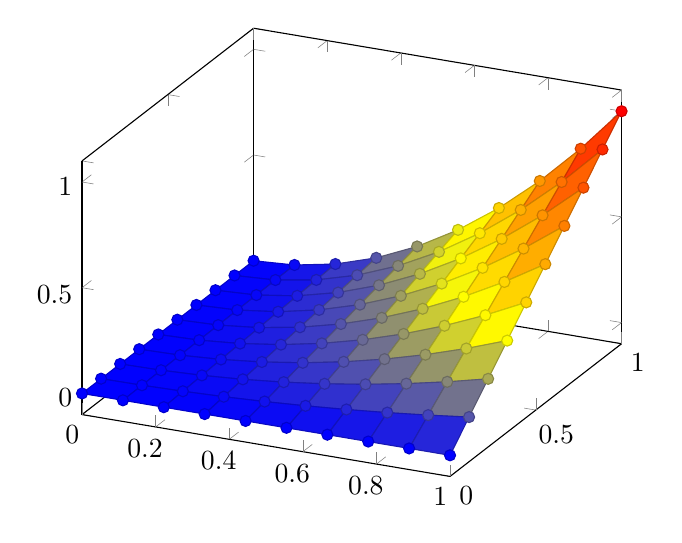
\begin{tikzpicture}
	\begin{axis}
	\addplot3[surf,shader=faceted,
		scatter,mark=*,
		samples=10,domain=0:1] 
		{x^2*y};
	\end{axis}
\end{tikzpicture}
\end{codeexample}
\end{pgfplotskey}

\begin{pgfplotskey}{faceted color=\marg{color name} (initially mapped color!80!black)}
	Defines the color to be used for meshes of faceted surface plots.

	Set |faceted color=none| to disable edge colors.
\end{pgfplotskey}

{
\tikzset{external/figure name/.add={}{interior_colormap_}}%
\tikzset{
	/pdflinks/search key prefixes in/.add={}{,/pgfplots/mesh/},
}%
\begin{pgfplotskeylist}{%
	mesh/interior colormap=\marg{map name}\marg{colormap specification},%
	mesh/interior colormap name=\marg{map name}}
	Allows to use a different |colormap| for the ``other side'' of the surface.

	Each mesh has two sides: one which ``points'' to the view's origin and one which points away from it. This key allows to define a second |colormap| for the side which points away from the view's origin. The motivation is to distinguish between the outer side and the interior parts of a surface:
\pgfplotsexpensiveexample
\begin{codeexample}[]
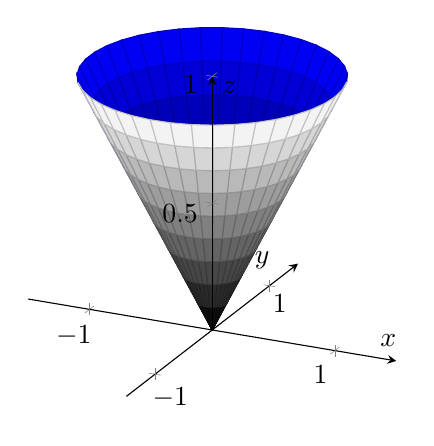
\begin{tikzpicture}
\begin{axis}[
  axis lines=center,
  axis on top,
  xlabel={$x$}, ylabel={$y$}, zlabel={$z$},
  domain=0:1,
  y domain=0:2*pi,
  xmin=-1.5, xmax=1.5,
  ymin=-1.5, ymax=1.5, zmin=0.0,
  mesh/interior colormap=
  	{blueblack}{color=(black) color=(blue)},
  colormap/blackwhite, 
  samples=10,
  samples y=40,
  z buffer=sort,
 ]
  \addplot3[surf] 
  	({x*cos(deg(y))},{x*sin(deg(y))},{x});
\end{axis}
\end{tikzpicture}
\end{codeexample}

	\noindent The |interior colormap| is often the one for the ```inner side''. However, the orientation of the surface depends on its normal vectors: \PGFPlots\ computes them using the right-hand-rule. The right-hand-rule applied to a triangle means to take the first encountered point, point the thumb in direction of the second point and the first finger in direction of the third point. Then, the normal for that triangle is the third finger (i.e.\ the cross--product of the involved oriented edges). For rectangular patches, \PGFPlots\ uses the normal of one of its triangles\footnote{This may change in future versions.}. Consequently, |mesh/interior colormap| will only work if the involved patch segments are consistently oriented. 
	
	A patch whose normal vector points into the same direction as the view direction uses the standard |colormap name|. A patch whose normal vector points into the opposite direction (i.e.\ in direction of the viewport) uses |mesh/interior colormap|.

\pgfplotsexpensiveexample
\begin{codeexample}[]
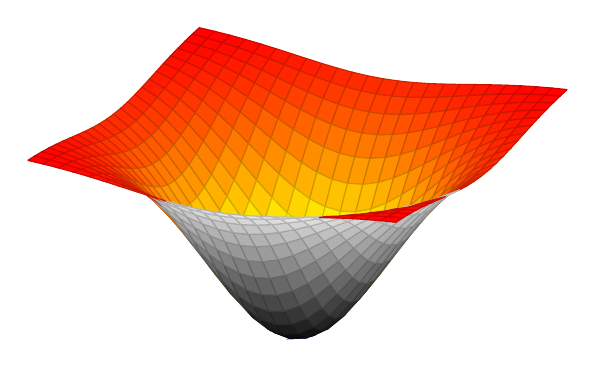
\begin{tikzpicture}
\begin{axis}[
  	hide axis,
	xlabel=$x$,ylabel=$y$,
	mesh/interior colormap name=hot,
	colormap/blackwhite, 
 ]
  \addplot3[domain=-1.5:1.5,surf]
  	{-exp(-x^2-y^2)};
\end{axis}
\end{tikzpicture}
\end{codeexample}

	The implementation of |mesh/interior colormap| works well for most examples; in particular, if the number of samples is large enough to resolve the boundary between inner and outer colormap. However, it might still produce spurious artifacts:
\pgfplotsexpensiveexample
\begin{codeexample}[]
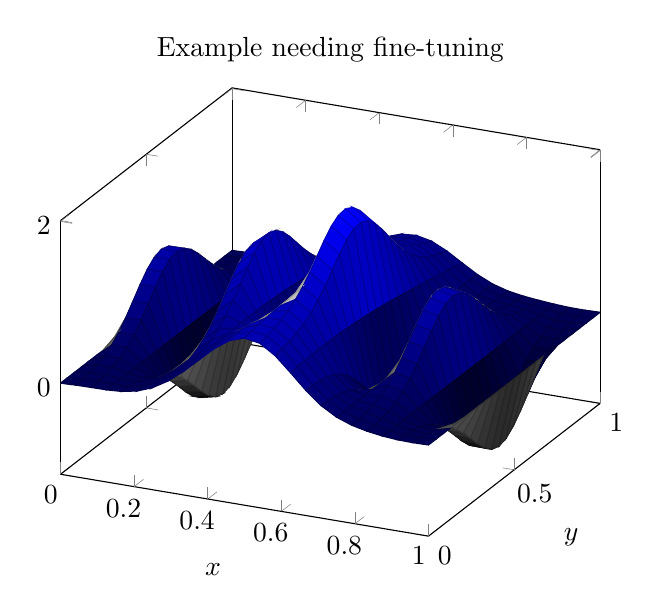
\begin{tikzpicture}
\begin{axis}[
	title=Example needing fine-tuning,
	xlabel=$x$,
	ylabel=$y$]
\addplot3[surf,
  mesh/interior colormap=
    {blueblack}{color=(black) color=(blue)},
  colormap/blackwhite, 
  domain=0:1] 
	{sin(deg(8*pi*x))* exp(-20*(y-0.5)^2) 
	+ exp(-(x-0.5)^2*30 
		- (y-0.25)^2 - (x-0.5)*(y-0.25))};
\end{axis}
\end{tikzpicture}
\end{codeexample}
	\noindent The previous example has need for improvement with respect to a couple of aspects: first, it has small overshoots near some of the meshes vertices (especially on top of the hills). These can be fixed using |miter limit=1|. Second, the boundary between blue and black is incorrect. This can be improved by means of an increased sampling density (|samples=31|). In addition, we can configure \PGFPlots\ to move the boundary between the two colormaps in favor of the blue region using |mesh/interior colormap thresh| as follows:
\pgfplotsexpensiveexample
\begin{codeexample}[]
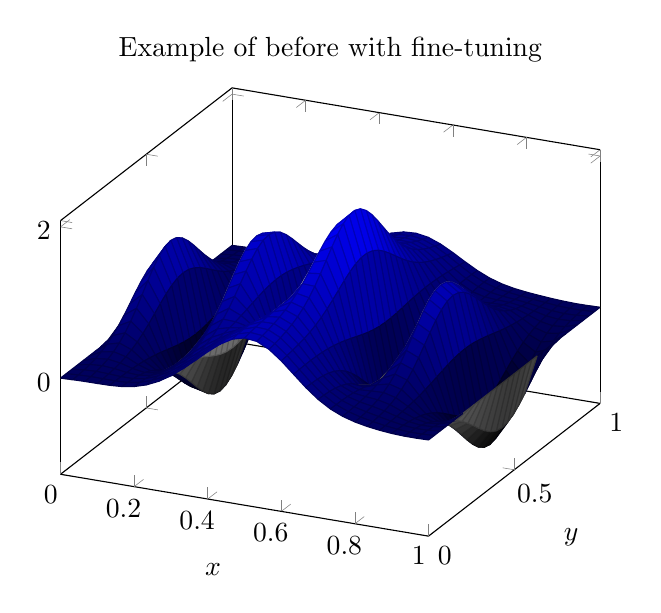
\begin{tikzpicture}
\begin{axis}[
	title=Example of before with fine-tuning,
	xlabel=$x$,
	ylabel=$y$]
\addplot3[surf,
  mesh/interior colormap=
    {blueblack}{color=(black) color=(blue)},
  % slightly increase sampling quality (was 25):
  samples=31,    
  % avoids overshooting corners:
  miter limit=1, 
  % move boundary between inner and outer:
  mesh/interior colormap thresh=0.1,
  colormap/blackwhite, 
  domain=0:1] 
	{sin(deg(8*pi*x))* exp(-20*(y-0.5)^2) 
	+ exp(-(x-0.5)^2*30 
		- (y-0.25)^2 - (x-0.5)*(y-0.25))};
\end{axis}
\end{tikzpicture}
\end{codeexample}
	\noindent This improves the display.
	\paragraph{Call for volunteers:} it would be nice if the fine--tuning of these keys would be unnecessary. If someone has well--founded suggestions (like knowledge and perhaps exhaustive experiments) on how to improve the feature, let me know.

	Note that |mesh/interior colormap| cannot be combined with |mesh/refines| currently.
	
	Note that |mesh/interior colormap| will increase compilation times due to the computation of normal vectors.
\end{pgfplotskeylist}

\begin{pgfplotskey}{mesh/interior colormap thresh=\marg{Number between $-1.0$ and $+1.0$} (initially 0)}
	A threshold which moves the boundary between the |colormap| and |interior colormap| in favor of |colormap| (if the value is negative) or in favor of |interior colormap| (if the value is positive). 
	
	The extreme value $-1$ essentially deactivates |interior colormap| whereas the other extreme $+1$ deactivates |colormap|.

	See above for an example.
\end{pgfplotskey}
}%

\begin{pgfplotskey}{surf shading/precision=\mchoice{pdf,postscript,ps} (initially postscript)}
	A key to configure how the low level driver for |shader=interp| writes its data. The choice |pdf| uses 32~bit binary coordinates (which is lossless). The resulting |.pdf| files appear to be correct, but they can't be converted to postscript -- the converter software always complains about an error. 

	The choice |postscript| (or, in short, |ps|) uses 24~bit truncated binary coordinates. This results in both, readable |.ps| and |.pdf| files. However, the truncation is lossy.

	If anyone has ideas how to fix this problem: let me know. As far as I know, Postscript should accept 32~bit coordinates, so it might be a mistake in the shading driver.
\end{pgfplotskey}

\subsubsection{Contour Plots}
{
\tikzset{external/figure name/.add={}{contour_}}%
\PGFPlots\ supports visualization of contour plots whose coordinates have been computed by \emph{external tools}. The |contour prepared| plot handler coming with \PGFPlots\ takes precomputed contour line coordinates and handles their visualization (|contour/draw color|, |contour/labels| etc.). The |contour gnuplot| style takes matrix input in the same format as for |mesh| or |surf| (that includes any of the \PGFPlots\ matrix input methods). It then writes the matrix data to a file and invokes |gnuplot| (or other, user customizable external programs) to compute contour coordinates. Finally, the computed contours are visualized with the |contour prepared| algorithm. Thus, external programs need to compute the contour coordinates and \PGFPlots\ visualizes the result.

We discuss the high level interface to external programs first and continue with |contour prepared| later-on.

\begin{plottype}[/pgfplots]{contour gnuplot=\textcolor{black}{\marg{{\normalfont options with `\texttt{contour/}' or `\texttt{contour external/}' prefix}}}}
	This is a high level contour plot interface. It expects matrix data in the same way as two dimensional |surf| or |mesh| plots do. It then computes contours and visualizes them.
\pgfplotsexpensiveexample
\begin{codeexample}[]
\begin{tikzpicture}
	\begin{axis}[view={0}{90}]
	\addplot3[contour gnuplot]
		{x*y};
	\end{axis}
\end{tikzpicture}
\end{codeexample}
	\noindent The example uses \verbpdfref{\addplot3} together with |expression| plotting, that means the input data is of the form $(x_i,y_i,f(x_i,y_i))$. The |view={0}{90}| flag means ``view from top'', otherwise the contour lines would have been drawn as $z$ value:
\pgfplotsexpensiveexample
\begin{codeexample}[]
\begin{tikzpicture}
	\begin{axis}
	\addplot3[contour gnuplot]
		{exp(0-x^2-y^2)};
	\end{axis}
\end{tikzpicture}
\end{codeexample}

As mentioned, you can use any of the \PGFPlots\ input methods as long as it yields matrix output. Thus, we can re-use our introductory example of matrix data, this time with inline data:
\pgfplotsexpensiveexample
\begin{codeexample}[]%
\begin{tikzpicture}%
	\begin{axis}[view={0}{90}]%
	\addplot3[contour gnuplot]%
		coordinates {
			(0,0,0) (1,0,0)   (2,0,0)   (3,0,0)

			(0,1,0) (1,1,0.6) (2,1,0.7) (3,1,0.5)

			(0,2,0) (1,2,0.7) (2,2,0.8) (3,2,0.5)
		};
	\end{axis}%
\end{tikzpicture}%
\end{codeexample}
	\noindent 

	What happens behind the scenes is that \PGFPlots\ takes the input matrix and writes all encountered coordinates to a temporary file, including the end--of--scanline markers. Then, it generates a small |gnuplot| script and invokes |gnuplot| to compute the contour coordinates, writing everything into a temporary output file. Afterwards, it includes |gnuplot|'s output file just as if you'd write |\addplot3[contour prepared] file |\marg{temporaryfile}|;|.

	All this invocation of |gnuplot|, including input/output file management is transparent to the user. It only requires two things: first of all, it requires matrix data as input\footnote{Note that \texttt{contour gnuplot} processes the input stream only once. Consequently, the temporary file will contain only information which was available before the first point has been seen. The example above works because it contains |empty line|s as end-of-scanline markers. If you do not provide such markers, you may need to provide two of the three options \texttt{mesh/rows}, \texttt{mesh/cols}, or \texttt{mesh/num points}.}. Second, it requires you to enable system calls. Consider the documentation for \verbpdfref{plot gnuplot} for how to enable system calls.

	Note that the $z$ coordinate of the data which is communicated to |gnuplot| is the current value of |point meta|. This allows to generate contours on two columns only and has more freedom. See also the |contour external/output point meta| key.

	There are several fine-tuning parameters of the input/output file management, and it is even possible to invoke different programs than |gnuplot| (even |matlab|). These details are discussed at the end of this section, see below at page~\pageref{key:pgfplots:contour:gnuplot}.
\end{plottype}

\begin{pgfplotskey}{contour/number=\marg{integer} (initially 5)}
	Configures the number of contour lines which should be produced by any external contouring algorithm.	
\pgfplotsexpensiveexample
\begin{codeexample}[]
\begin{tikzpicture}
    \begin{axis}[
        title={$x \exp(-x^2-y^2)$},
		domain=-2:2,enlarge x limits,
        view={0}{90},
    ]
   \addplot3[contour gnuplot={number=14},thick]
          {exp(0-x^2-y^2)*x};
    \end{axis}
\end{tikzpicture}
\end{codeexample}
	It is also possible to change the |/pgf/number format| settings, see the documentation for the |contour/every contour label| style below.


	Note that |contour/number| has no effect on |contour prepared|.
\end{pgfplotskey}

\begin{pgfplotskey}{contour/levels=\marg{list of levels} (initially empty)}
	Configures the number of contour lines which should be produced by any external contouring algorithm by means of a list of discrete levels.
\pgfplotsexpensiveexample
\begin{codeexample}[]
\begin{tikzpicture}
    \begin{axis}[
        title={$x \exp(-x^2-y^2)$},
		domain=-2:2,
		enlargelimits,
        view={0}{90},
    ]
   \addplot3[
     contour gnuplot={levels={-0.1,-0.2,-0.6}},
   	 thick]
          {exp(0-x^2-y^2)*x};
    \end{axis}
\end{tikzpicture}
\end{codeexample}
	It is also possible to change the |/pgf/number format| settings, see the documentation for the |contour/every contour label| style below.

	This key has higher precedence than |contour/number|, i.e.\ if both are given, |contour/levels| will be active.

	Note that |contour/levels| has no effect on |contour prepared|.
\end{pgfplotskey}

\begin{plottype}[/pgfplots]{contour prepared=\textcolor{black}{\marg{{\normalfont options with `\texttt{contour/}' prefix}}}}
	A plot handler which expects already computed contours on input and visualizes them. It cannot compute contours on its own.

	\begin{pgfplotskey}{contour prepared format=\mchoice{standard,matlab} (initially standard)}
	There are two accepted input formats. The first is a long sequence of coordinates of the form $(x,y,z)$ where all successive coordinates with the same $z$ value make up a contour level (this is only part of complete truth, see below). The end--of--scanline markers (|empty line|s in the input) mark an interruption in one contour level.

	For example, |contour prepared format=standard| could be\footnote{This is actually the output from our \texttt{\textbackslash addplot3[contour gnuplot] coordinates} example from above.}
\begin{codeexample}[]
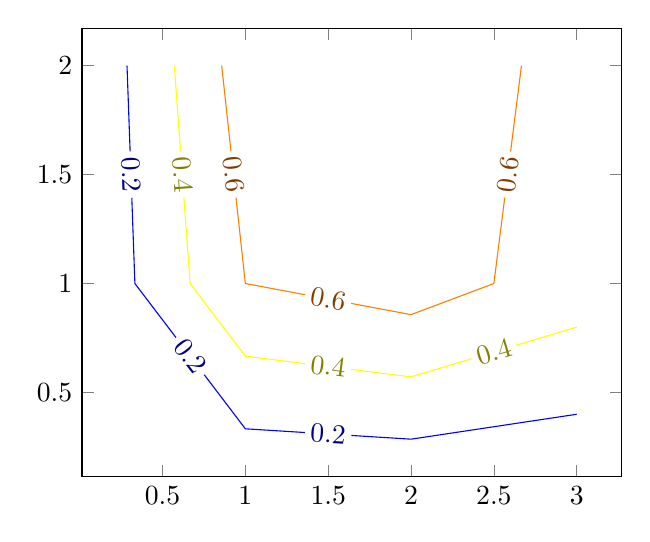
\begin{tikzpicture}
	\begin{axis}
	\addplot[contour prepared]
		table {
			 2  2  0.8        
			                  
			 0.857143  2  0.6 
			 1  1  0.6        
			 2  0.857143  0.6 
			 2.5  1  0.6      
			 2.66667  2  0.6  
			                  
			 0.571429  2  0.4 
			 0.666667  1  0.4 
			 1  0.666667  0.4 
			 2  0.571429  0.4 
			 3  0.8  0.4      
			                  
			 0.285714  2  0.2 
			 0.333333  1  0.2 
			 1  0.333333  0.2 
			 2  0.285714  0.2 
			 3  0.4  0.2      
		};
	\end{axis}
\end{tikzpicture}
\end{codeexample}
	\noindent Note that the |empty line|s are not necessary in this case: |empty line|s make only a difference if they occur within the same contour level (i.e. if the same $z$ value appears above and below of them).
		
		The choice |contour prepared format=matlab| expects two--dimensional input data where the contour level and the number of elements of the contour line are provided as $x$ and $y$ coordinates, respectively, of a leading point. Such a format is used by |matlab|'s contour algorithms, i.e.\ it resembles the output of the matlab commands |data=contour(...)| or |data=contourc(...)|.

% I generates the following example with plotdata/pgfplotscontourmatlabexample.m

\begin{codeexample}[]
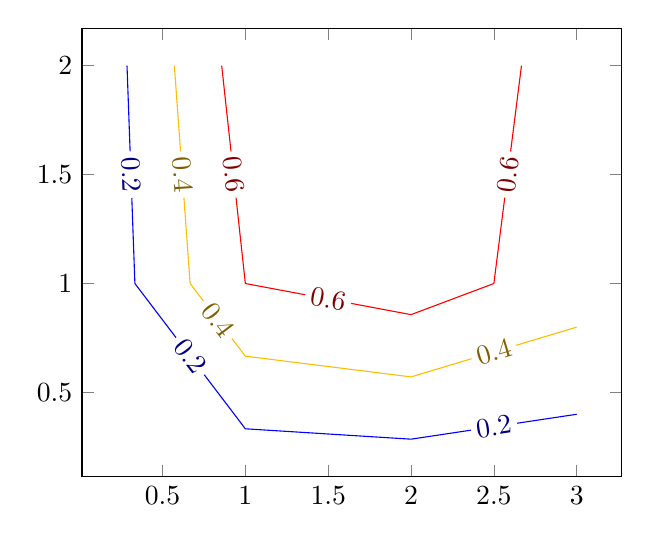
\begin{tikzpicture}
	\begin{axis}
	\addplot[contour prepared,
		contour prepared format=matlab]
	table {
% (0.2,5) ==> contour `0.2' (x), 5 points follow (y):
	   2.0000000e-01   5.0000000e+00 
	   3.0000000e+00   4.0000000e-01 
	   2.0000000e+00   2.8571429e-01 
	   1.0000000e+00   3.3333333e-01 
	   3.3333333e-01   1.0000000e+00 
	   2.8571429e-01   2.0000000e+00 
% (0.4,5) ==> contour `0.4', consists of 5 points
	   4.0000000e-01   5.0000000e+00 
	   3.0000000e+00   8.0000000e-01 
	   2.0000000e+00   5.7142857e-01 
	   1.0000000e+00   6.6666667e-01 
	   6.6666667e-01   1.0000000e+00 
	   5.7142857e-01   2.0000000e+00 
% (0.6,6) ==> contour `0.6', has 6 points
	   6.0000000e-01   6.0000000e+00 
	   2.6666667e+00   2.0000000e+00 
	   2.5000000e+00   1.0000000e+00 
	   2.0000000e+00   8.5714286e-01 
	   1.0000000e+00   1.0000000e+00 
	   1.0000000e+00   1.0000000e+00 
	   8.5714286e-01   2.0000000e+00 
		};
	\end{axis}
\end{tikzpicture}
\end{codeexample}

		In case you use matlab, you can generate such data with
\begin{verbatim}
[x,y]=meshgrid(linspace(0,1,15));
data=contour(x,y,x.*y);
data=data';
save 'exporteddata.dat' data -ASCII
\end{verbatim}
	\end{pgfplotskey}

	As already mentioned in the beginning, the $z$ coordinate is not necessarily the coordinate used to delimit contour levels. In fact, the |point meta| data is acquired here, i.e.\ you are free to use whatever $z$ coordinate you want as long as you have a correct |point meta| value. The example from above could be modified as follows:
\begin{codeexample}[]
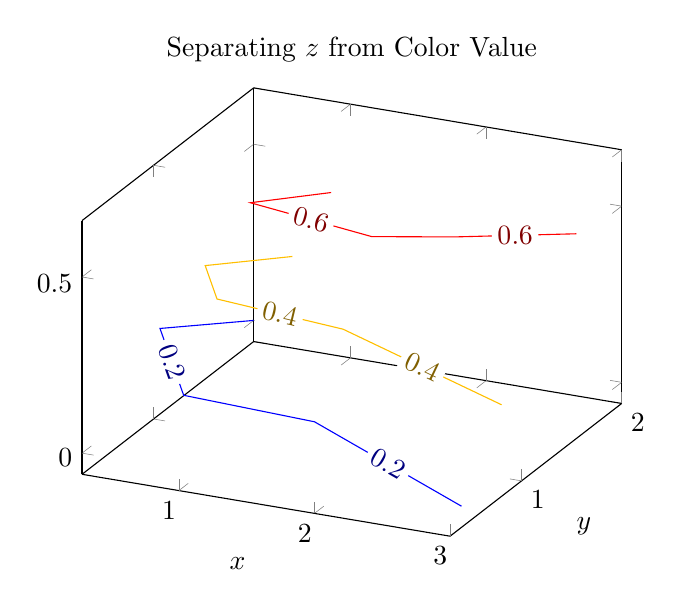
\begin{tikzpicture}
	\begin{axis}[
		title=Separating $z$ from Color Value,
		xlabel=$x$,
		ylabel=$y$,
	]
	\addplot3[contour prepared,
		point meta=\thisrow{level}]
		table {
	 x         y   z   level   
	 0.857143  2  0.4 0.6		
	 1         1  0.6  0.6		
	 2  0.857143 0.6  0.6		
	 2.5  1      0.6  0.6		
	 2.66667  2  0.4  0.6		
	                  		
	 0.571429  2  0.2 0.4		
	 0.666667  1  0.4 0.4		
	 1  0.666667  0.4 0.4		
	 2  0.571429  0.4 0.4		
	 3  0.8       0.2 0.4		
	                  		
	 0.285714  2  0   0.2		
	 0.333333  1  0.2 0.2		
	 1  0.333333  0.2 0.2		
	 2  0.285714  0.2 0.2		
	 3  0.4       0   0.2		
		};
	\end{axis}
\end{tikzpicture}
\end{codeexample}
	\noindent The example above uses different $z$ coordinates for each first and each last point on contour lines. The contour lines as such are defined by the |level| column since we wrote |point meta=\thisrow{level}|. Such a feature also allows |contour prepared| for nonstandard axes, compare the examples for the |ternary| lib on page~\pageref{page:ternary:contour}.

	\begin{pgfplotskey}{contour/draw color=\marg{color} (initially mapped color)}
		Defines the draw color for every contour. Note that only |mapped color| actually depends on the contour level.
	\end{pgfplotskey}

	\begin{pgfplotskey}{contour/labels=\marg{true,false} (initially true)}
		Configures whether contour labels shall be drawn or not.
	\end{pgfplotskey}
	\begin{pgfplotskey}{contour/label distance=\marg{dimension} (initially 70pt)}
		Configures the distance between adjacend contour labels within the same contour level.
	\end{pgfplotskey}

	\begin{stylekey}{/pgfplots/contour/every contour label}
		Allows to customize contour labels. The preferred way to change this style is the |contour label style=|\marg{options} method, see below.

		The initial value is
\begin{codeexample}[code only]
\pgfplotsset{
	contour/every contour label/.style={
		sloped,
		transform shape,
		inner sep=2pt,
		every node/.style={mapped color!50!black,fill=white},
		/pgf/number format/relative={\pgfplotspointmetarangeexponent},
	}
}
\end{codeexample}
	\noindent Note that |\pgfplotspointmetarangeexponent|$=e$ where $\pm m \cdot 10^e$ is the largest occuring label value (technically, it is the largest occurring value of |point meta|).

		The following example modifies the |/pgf/number format| styles for contour labels:
\begin{codeexample}[]
\begin{tikzpicture}
    \begin{axis}[
        title={$x \exp(-x^2-y^2)$},
		domain=-2:2,enlarge x limits,
        view={0}{90},
    ]
   \addplot3[
   		contour gnuplot={
			scanline marks=required,
   			number=14,
			contour label style={
				/pgf/number format/fixed,
				/pgf/number format/precision=1,
			},
		},thick
	]
          {exp(0-x^2-y^2)*x};
    \end{axis}
\end{tikzpicture}
\end{codeexample}
	\end{stylekey}
	
\pgfplotsshortstylekey contour/contour label style=contour/every contour label\pgfeov
	\begin{stylekey}{/pgfplots/contour/labels over line}
		A style which changes |every contour label| such that labels are right over the lines, without fill color.

\begin{codeexample}[]
\begin{tikzpicture}
	\begin{axis}[view={0}{90}]
	\addplot3[contour gnuplot={
		labels over line,number=9}]
		{x*y};
	\end{axis}
\end{tikzpicture}
\end{codeexample}
	\end{stylekey}

	\begin{stylekey}{/pgfplots/contour/handler}
		Allows to modify the plot handler which connects the points of a single contour level.

		The initial value is 
\begin{codeexample}[code only]
\pgfplotsset{contour/handler/.style={/tikz/sharp plot}}
\end{codeexample}
		but a useful alternative might be the |smooth| handler.
	\end{stylekey}

	\begin{pgfplotscodekey}{contour/label node code}
		A lowlevel interface to modify how contour labels are placed.

		The initial value is
\begin{codeexample}[code only]
\pgfplotsset{
	contour/label node code/.code={\node {\pgfmathprintnumber{#1}};}
}
\end{codeexample}
	\end{pgfplotscodekey}

\end{plottype}


\begin{plottype}[/pgfplots]{contour external=\textcolor{black}{\marg{{\normalfont options with `\texttt{contour/}' or `\texttt{contour external/}' prefix}}}}
	This handler constitutes a generic interface to external programs to compute contour lines. The |contour gnuplot| method is actually a special case of |contour external|.

	\begin{pgfplotskey}{contour external/file=\marg{base file name} (initially empty)}
		The initial configuration is to automatically generate a unique file name.
	\end{pgfplotskey}

	\begin{pgfplotskey}{contour external/scanline marks=\mchoice{false,if in input,required,true} (initially if in input)}
		Controls how |contour external| writes end-of-scanline markers. 

		The choice |false| writes no such markers at all. In this case, |script| should contain |mesh/rows| and/or |mesh/cols|.

		The choice |if in input| generates end-of-scanline markers if they appear in the provided input data (either as |empty line|s or if the user provided at least two of the three options |mesh/rows|, |mesh/cols|, or |mesh/num points| explicitly).

		The choice |required| works like |if in input|, but it will fail unless there really was such a marker.

		The choice |true| is an alias for |required|.
	\end{pgfplotskey}

	\begin{pgfplotskey}{contour external/script=\marg{Code for external program} (initially empty)}
		Provides template code to generate a script for the external program. Inside of \meta{Code for external program}, the placeholder |\infile| will expand to the temporary input file and |\outfile| to the temporary output file. The temporary |\infile| is a text file containing one point on each line, in the form |x y meta meta|, separated by tabstops. Whenever a scanline is complete, an |empty line| is issued (but only if these scanline markers are found in the input stream as well). The complete set of scanlines forms a matrix. There are no additional comments or extra characters in the file. The macro |\ordering| will expand to |0| if the matrix is stored in |mesh/ordering=x varies| and |\ordering| will be |1| for |mesh/ordering=y varies|.

		Inside of \meta{Code for external program}, you can also use |\pgfkeysvalueof{/pgfplots/mesh/rows}| and |\pgfkeysvalueof{/pgfplots/mesh/cols}|; they expand to the matrix' size. Similarly, |\pgfkeysvalueof{/pgfplots/mesh/num points}| expands to the total number of points.

		Inside of \meta{Code for external program}, the macro \declareandlabel{\thecontournumber} is defined to be the value |\pgfkeysvalueof{/pgfplots/contour/number}| and \declareandlabel{\thecontourlevels} contains the value |\pgfkeysvalueof{/pgfplots/contour/levels}|. These two macros simplify conditional code.

		If you need one of the characters [\verb!"|;:#'`!] and some macro package already uses the character for other purposes, you can prepend them with a backslash, i.e. write |\"| instead of |"|.
	\end{pgfplotskey}

	\begin{pgfplotskey}{contour external/script extension=\marg{extension} (initially script)}
		The file name extension for the temporary script.
	\end{pgfplotskey}

	\begin{pgfplotskey}{contour external/cmd=\marg{system call} (initially empty)}
		A template to generate system calls for the external program. Inside of \meta{system call}, you may use |\script| as placeholder for the filename which contains the result of |contour external/script|.
	\end{pgfplotskey}

	\begin{pgfplotskey}{contour external/output point meta=\marg{point meta read from result of external tool} (initially empty)}
		Allows to customize the |point meta| configuration which is applied to the result of the external tool.

		In |contour external|, the value of |point meta| is used to generate the \emph{input} $z$ coordinate for the external tool.

		As soon as the external tool computed contour lines, its output is read and interpreted as contour lines -- and the value of |output point meta| determines the value of |point meta| which will be used to visualize the result. 

		An empty value means to use the $z$ coordinate returned by the external tool.

		Any other value is interpreted as a valid choice of |point meta|.
	\end{pgfplotskey}

	\begin{stylekey}{/pgfplots/contour gnuplot}
		\label{key:pgfplots:contour:gnuplot}
		The initial configuration is
\begin{codeexample}[code only]
\pgfplotsset{
	contour gnuplot/.style={
		contour external={
			script={
				unset surface; 
				\ifx\thecontourlevels\empty
				set cntrparam levels \thecontournumber;
				\else
				set cntrparam levels discrete \thecontourlevels;
				\fi
				set contour;
				set table \"\outfile\"; 
				splot \"\infile\";
			},
			cmd={gnuplot \"\script\"},
			#1,%
		},
	}
}
\end{codeexample}
	Note that |contour gnuplot| requires explicit scanline markers in the input stream, and it assumes |mesh/ordering=x varies|.
	\end{stylekey}

	Note that |contour external| lacks the intelligence to detect changes; it will always re-generate the output (unless the |-shell-escape| feature is not active).
\end{plottype}

%--------------------------------------------------
% \subsubsection{Filled Contours (Experimental)}
% Filled contour plots are \emph{not} ready yet. There is only limited experimental support up to now. Use at your own risk!
% 
% \begin{pgfplotskey}{contour/data limits={$(\underline x,\underline y,\underline z,\underline m)$ $(\bar x,\bar y,\bar z,\bar m)$} (initially empty)}
% 	The data limits for $x$, $y$, $z$ and |point meta|, separated by comma.
% \end{pgfplotskey}
% 
% \begin{pgfplotskey}{contour/filled=\mchoice{true,false} (initially false)}
% 	A boolean which configures the (highly experimental) feature to fill any |contour prepared| plot.
% \end{pgfplotskey}
% \begin{pgfplotskey}{contour/fill color=\marg{color} (initially mapped color)}
% 	Designates the fill color. Use something like |fill color=mapped color!80!black| if you want to distinguish between edges and filled area.
% \end{pgfplotskey}
%-------------------------------------------------- 

}

\subsubsection{Parameterized Plots}
Parameterized plots use the same plot types as documented in the preceding sections: both |mesh| and |surf|ace plots are actually special parametrized plots where $x$ and $y$ are on cartesian grid points.

Parameterized plots just need a special way to provide the coordinates:

\pgfplotsexpensiveexample
\begin{codeexample}[]
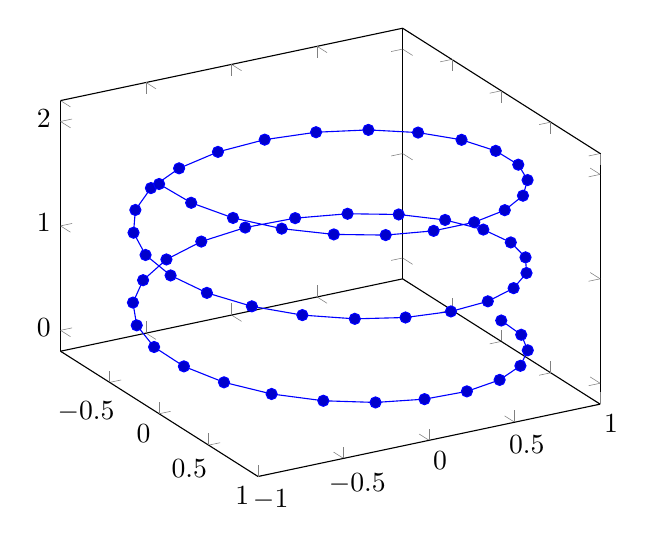
\begin{tikzpicture}
	\begin{axis}[view={60}{30}]
	\addplot3+[domain=0:5*pi,samples=60,samples y=0] 
		({sin(deg(x))},
		 {cos(deg(x))},
		 {2*x/(5*pi)});
	\end{axis}
\end{tikzpicture}
\end{codeexample}
\noindent The preceding example uses |samples y=0| to indicate that a line shall be sampled instead of a matrix. The curly braces are necessary because \TeX\ can't nest round braces. The single expressions here are used to parametrize the helix.

Another example follows. Note that |z buffer=sort| is a necessary method here.

\pgfplotsexpensiveexample
\begin{codeexample}[]
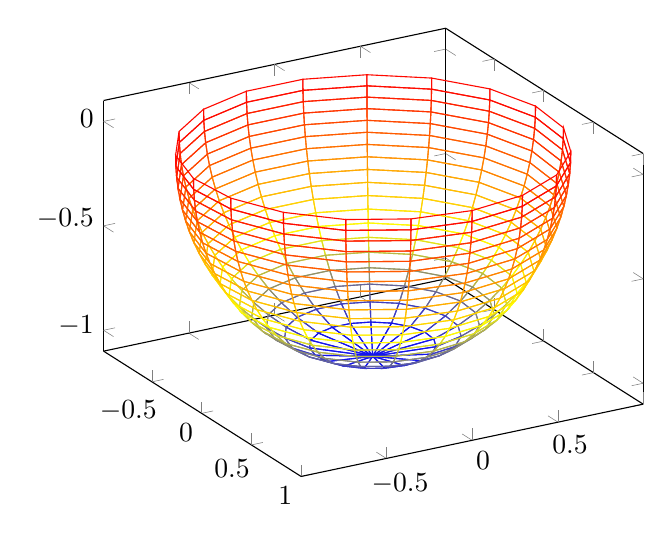
\begin{tikzpicture}
\begin{axis}[view={60}{30}]
	\addplot3[mesh,z buffer=sort,
		samples=20,domain=-1:0,y domain=0:2*pi]
		({sqrt(1-x^2) * cos(deg(y))},
		 {sqrt( 1-x^2 ) * sin(deg(y))},
		 x);
\end{axis}
\end{tikzpicture}
\end{codeexample}

\pgfplotsexpensiveexample
\begin{codeexample}[]
\begin{tikzpicture}
\begin{axis}[view={60}{30}]
	\addplot3[mesh,z buffer=sort,
		scatter,only marks,scatter src=z,
		samples=30,domain=-1:1,y domain=0:2*pi]
		({sqrt(1-x^2) * cos(deg(y))},
		 {sqrt( 1-x^2 ) * sin(deg(y))},
		 x);
\end{axis}
\end{tikzpicture}
\end{codeexample}

\pgfplotsexpensiveexample
\begin{codeexample}[]
\begin{tikzpicture}
\begin{axis}[view={60}{30}]
	\addplot3[surf,shader=interp,z buffer=sort,
		samples=30,domain=-1:0,y domain=0:2*pi]
		({sqrt(1-x^2) * cos(deg(y))},
		 {sqrt( 1-x^2 ) * sin(deg(y))},
		 x);
\end{axis}
\end{tikzpicture}
\end{codeexample}

\subsubsection{3D Quiver Plots (Arrows)}
Three dimensional |quiver| plots are possible with the same interface as their two-dimensional counterparts, simply provide the third coordinate using |quiver/w|. Please refer to Section~\ref{sec:pgfplots:quiver2d} for details and examples.

\subsubsection{About 3D Const Plots and 3D Bar Plots}
There are currently \emph{no} equivalents of |const plot| and its variants or the bar plot types like |ybar| for three dimensional axes, sorry.

\subsubsection{Patch Plots}
\label{sec:pgfplots:3d:patch}
\begin{plottype}[/pgfplots]{patch}
	Patch plots are similar to |mesh| and |surf| plots in that they describe a filled area by means of a geometry.

	However, |patch| plots are defined by \emph{explicitly} providing the elements of the geometry: they expect a sequence of triangles (or other |patch type|s) which make up the mesh.

	There are two dimensional and three dimensional patch plots, both with the same interfaces which are explained in the following sections.

	The standard input format (constituted by |mesh input=patches|) is to provide a sequence of coordinates (either two-- or three--dimensional) as usual. Each consecutive set of points makes up a patch element, which is often a triangle:
\begin{codeexample}[]
\begin{tikzpicture}
	\begin{axis}
	\addplot[patch]
	table {
		x y 
		0 0 
		1 1 
		2 0
% empty lines do not hurt, they are ignored here:

		1 1 
		2 0 
		3 1 
		
		2 0 
		3 1 
		4 0 
		
	};
	\end{axis}
\end{tikzpicture}
\end{codeexample}
	\noindent Patch plots use |point meta| to determine fill colors. In its initial configuration, |point meta| will be set to the $y$ coordinate (or the $z$ coordinate for three dimensional |patch| plots). Set |point meta| somehow to color the patches:
\begin{codeexample}[]
\begin{tikzpicture}
	\begin{axis}
	\addplot[patch]
	table[point meta=\thisrow{c}] {
		x y c
		0 0 0.2
		1 1 0
		2 0 1
		
		1 1 0
		2 0 1
		3 1 0
		
		2 0 1
		3 1 0
		4 0 0.5
	};
	\end{axis}
\end{tikzpicture}
\end{codeexample}
	Patch plots make use of the |mesh| configuration, including the |shader|. Thus, the example above uses the initial |shader=faceted| (which uses the \emph{mean} color data to determine a triangle's color and a related stroke color). The |shader=interp| yields the following result:
\begin{codeexample}[]
\begin{tikzpicture}
	\begin{axis}
	\addplot[patch,shader=interp]
	table[point meta=\thisrow{c}] {
		x y c
		0 0 0.2
		1 1 0
		2 0 1
		
		1 1 0
		2 0 1
		3 1 0
		
		2 0 1
		3 1 0
		4 0 0.5
	};
	\end{axis}
\end{tikzpicture}
\end{codeexample}
	\noindent For triangles, |shader=interp| results in linearly interpolated |point meta| values throughout each individual triangle, which are then mapped to the color map (a technique also known as Gouraud shading).

	The color data does not need to be continuous, it is associated to triangle vertices. Thus, changing some of the color values allows individually shaded regions:
\begin{codeexample}[]
\begin{tikzpicture}
	\begin{axis}
	\addplot[patch,shader=interp]
	table[point meta=\thisrow{c}] {
		x y c
		0 0 0.2
		1 1 0
		2 0 1
		
		1 1 0
		2 0 -1
		3 1 0
		
		2 0 0.5
		3 1 1
		4 0 0.5
	};
	\end{axis}
\end{tikzpicture}
\end{codeexample}
	
	Two dimensional |patch| plots simply draw triangles in their order of appearance. In three dimensions, single elements are sorted according to their view depth, with foreground elements drawn on top of background elements (``Painter's algorithm'', see |z buffer=sort|).

\begin{pgfplotskeylist}{%
	patch table=\marg{table file name or inline table} (initially empty),%
	patch table with point meta=\marg{table file name or inline table} (initially empty),%
	patch table with individual point meta=\marg{table file name or inline table} (initially empty)%
}
	Allows to provide patch connectivity data stored in an input table.

	A non--empty argument for |patch table| enables patch input mode. Now, the standard input stream is a long list of vertices which are stored in an array using their |\coordindex| as key. Each row of \meta{table file name or inline table} makes up one patch, defined by indices into the vertex array:
\begin{codeexample}[]
\begin{tikzpicture}
	\begin{axis}
	\addplot[patch,table/row sep=\\,patch table={%
		0 1 2\\
		1 2 3\\
		4 3 5\\
	}]
	table[row sep=\\,point meta=\thisrow{c}] {
		x y c  \\
		0 0 0.2\\% 0
		1 1 0  \\% 1
		2 0 1  \\% 2
		3 1 0  \\% 3
		2 0 0.5\\% 4
		4 0 0.5\\% 5
	};
	\end{axis}
\end{tikzpicture}
\end{codeexample}
	\noindent The example consists of \emph{two separate} tables. The |patch table| argument is a table, provided inline where rows are separated by |\\| (which is the purpose of the |row sep=\\| key as you guessed\footnote{Note that the choice \texttt{row sep=\textbackslash\textbackslash} is much more robust here: newlines would be converted to spaces by \TeX\ before \PGFPlots\ had a chance to see them.}). The |patch table| here declares three triangles: the triangle made up by vertex $\#0$, $\#1$ and $\#2$, the triangle made up by $\#1$, $\#2$ and $\#3$ and finally the one using the vertices $\#4$, $\#3$ and $\#5$. The vertices as such are provided using the standard input methods of \PGFPlots; in our case using a table as well. The standard input simply provides coordinates (and |point meta|) which are stored in the vertex array; you could also have used |plot coordinates| to provide them (or |plot expression|).
	
	The argument to |patch table| needs to be a table -- either a file name or an inline table as in the example above. The first $n$ columns of this table are assumed to contain indices into the vertex array (which is made up using all vertices of the standard input as explained in the previous paragraph). The entries in this table can be provided in floating point, just make sure they are not rounded. The variable $n$ is the number of vertices required to make up a single patch. For triangular patches, it is $n=3$, for |patch type=bilinear| it is $n=4$ and similar for other choices of |patch type|.

	The alternative \declaretext{patch table with point meta} is almost the same as |patch table| -- but it allows to provide (a single) |point meta| (color data) per patch instead of per vertex. Here, a further column of the argument table is interpreted as color data:
\begin{codeexample}[]
\begin{tikzpicture}
	\begin{axis}
	% this uses per-patch color data:
	\addplot[patch,table/row sep=\\,
	patch table with point meta={%
		0 1 2 100\\
		1 2 3 10\\
		4 3 5 0\\
	}]
	table[row sep=\\] {
		x y \\
		0 0 \\% 0
		1 1 \\% 1
		2 0 \\% 2
		3 1 \\% 3
		2 0 \\% 4
		4 0 \\% 5
	};
	\end{axis}
\end{tikzpicture}
\end{codeexample}
	\noindent The |patch table with point meta| always prefers |point meta| data from the provided table argument. However, it is still supported to write |point meta=\thisrow|\marg{colname} or similar constructs -- but now, \meta{colname} refers to the provided table argument. More precisely, |point meta| is evaluated in a context where the patch connectivity has been resolved and the |patch table with point meta| is loaded.

	The other alternative \declaretext{patch table with individual point meta} is very similar, but instead of a flat color per patch, it allows to write one color value for every patch:
\begin{codeexample}[]
\begin{tikzpicture}
	\begin{axis}
	% this uses n per-patch color values:
	\addplot[patch,shader=interp,
	table/row sep=\\,
	patch table with individual point meta={%
		0 1 2 100 100 100\\% V_0 V_1 V_2 C_0 C_1 C_2
		1 2 3 10 0 50\\
		4 3 5 0 0 100\\
	}]
	table[row sep=\\] {
		x y \\
		0 0 \\% 0
		1 1 \\% 1
		2 0 \\% 2
		3 1 \\% 3
		2 0 \\% 4
		4 0 \\% 5
	};
	\end{axis}
\end{tikzpicture}
\end{codeexample}
	\noindent To find the |point meta| data for vertex $\#i, i=0,1,2$, \PGFPlots\ searches in column $i+n$ where $n$ is the number of vertices for |patch type| (in our case, $n=3$). 
	
	Technical remark: The key |patch table with individual point meta| automatically installs |point meta=explicit| as well. It might be confusing to override the value of |point meta| here (although it is allowed). 

	The |patch table| input type allows to reduce the size of geometries since vertices are stored just once. \PGFPlots\ unpacks them into memory into the redundant format in order to work with single patch elements\footnote{The reason for such an approach is that \TeX\ doesn't really know what an array is -- and according to my experience, arrays implemented by macros tend to blow up \TeX's memory limits even faster than the alternative.}. In case you experience \TeX\ memory problems with this connectivity input, consider using the redundant format. It uses other types of memory limits.
	\index{Errors!Patch Input and Memory Problems}
\end{pgfplotskeylist}
	
	A more involved example is shown below; it uses |\addplot3[patch]| to visualize a three dimensional |patch| plot, provided by means of a long sequence of patches:
\pgfplotsexpensiveexample
\begin{codeexample}[]
\begin{tikzpicture}
\begin{axis}[axis equal]
% FokkerDrI_layer_0.patches.dat contains:
% # each row is one vertex; three consecutive 
% # vertices make one triangle (patch)
% 105.577	-19.7332	2.85249	
% 88.9233	-21.1254	13.0359	
% 89.2104	-22.1547	1.46467	
% # end of facet 0
% 105.577	-19.7332	2.85249	
% 105.577	-17.2161	12.146	
% 88.9233	-21.1254	13.0359	
% # end of facet 1
\addplot3[patch] 
	file
	{plotdata/FokkerDrI_layer_0.patches.dat};
\end{axis}
\end{tikzpicture}
\end{codeexample}
	\noindent The ordering in which triangles are specified is irrelevant, three--dimensional patch plots use |z buffer=sort| to sort patches according to their depth (defined as mean depth over each vertex), where foreground patches are drawn on top of background patches. This so--called ``Painter's algorithm'' works well for most meshes. If it fails, consider using |patch refines=1| or |patch refines=2| to split larger elements into small ones automatically.


	The drawing color associated to single vertices can be changed using the |point meta| key (which is the common method to configure color data in \PGFPlots). The initial configuration is |point meta=z| for three dimensional |patch| plots, i.e.\ to use the $z$ coordinate also as color data. Use |point meta=\thisrow|\marg{colname} in conjunction with |\addplot3[patch] table| to load a selected table column.

	Patch plots are (almost) the same as |mesh| or |surf| plots, they only have more freedom in their input format (and a more complicated geometry). Actually, ``|patch|'' is just a style for |surf,mesh input=patches|. In other words, |patch| \emph{is} the same as |surf|, it even shares the same internal implementation. Thus, most of the keys to configure |mesh| or |surf| plots apply to |patch| as well, especially |shader| and |z buffer|. As already mentioned, |\addplot3[patch]| automatically activates |z buffer=sort| to ensure a good drawing sequence. The |shader| can be used to modify the appearance:
\pgfplotsexpensiveexample
\begin{codeexample}[]
\begin{tikzpicture}
\begin{axis}
% FokkerDrI_layer_0.facetIdx.dat contains:
% # each row makes up one facet; it 
% # consists of 0-based indices into 
% # the vertex array
% 0	1	2 % triangle of vertices #0,#1 and #2
% 0	3	1 % triangle of vertices #0,#3 and #1	
% 3	4	1	
% 5	6	7	
% 6	8	7	
% 8	9	7	
% 8	10	9	
% ...
% while FokkerDrI_layer_0.vertices.dat contains
% 105.577	-19.7332	2.85249	% vertex #0
% 88.9233	-21.1254	13.0359	% vertex #1
% 89.2104	-22.1547	1.46467	% vertex #2
% 105.577	-17.2161	12.146	
% 105.577	-10.6054	18.7567	
% 105.577	7.98161	18.7567	
% 105.577	14.5923	12.146	
% ...
\addplot3[patch,shader=interp,
	patch table=
		{plotdata/FokkerDrI_layer_0.facetIdx.dat}] 
	file
	{plotdata/FokkerDrI_layer_0.vertices.dat};
\end{axis}
\end{tikzpicture}
\end{codeexample}
	See the description of |shader=interp| for details and remarks. The example above makes use of the alternative syntax to provide a geometry: the |patch table| input. It allows to provide vertices separate from patch connectivity, where each patch is defined using three indices into the vertex array as discussed above.

\pgfplotsexpensiveexample
\begin{codeexample}[]
\begin{tikzpicture}
\begin{axis}[view/h=70]
% FokkerDrI_layer_0.patches.dat contains:
% # each row is one vertex; three consecutive 
% # vertices make one triangle (patch)
% 105.577	-19.7332	2.85249	
% 88.9233	-21.1254	13.0359	
% 89.2104	-22.1547	1.46467	
% # end of facet 0
% 105.577	-19.7332	2.85249	
% 105.577	-17.2161	12.146	
% 88.9233	-21.1254	13.0359	
% # end of facet 1
\addplot3[patch,mesh] 
	file
	{plotdata/FokkerDrI_layer_0.patches.dat};
\end{axis}
\end{tikzpicture}
\end{codeexample}

\begin{pgfplotskey}{mesh input=\mchoice{lattice,patches}}
	This key controls how input coordinates are decoded to get patches. It is used only if |patch table| is empty (|patch table| has its own way to decode input coordinates). Usually, you won't need to bother with this key as it is set implicitly.

	The choice |mesh input=lattice| is the initial configuration for |mesh| and |surf| plots: it expects input in a compact matrix form as described at the beginning of this section starting with page~\pageref{sec:3d} and requires a |mesh/ordering| and perhaps end--of--scanline markers. It yields patches with exactly four corners and is compatible with |patch type=rectangle| and |patch type=bilinear| (the latter requiring to load the |patchplots| library).

	The choice |mesh input=patches| is implicitly set when you use the |patch| style (remember that |surf| is actually some sort of patch plot on its own). It expects the input format as described for |patch| plots, i.e.\ $n$ consecutive coordinates make up the vertices of a single patch where $n$ is the expected number of vertices for the configured |patch type|. 

	Note that a non--empty |patch table| implies |mesh input=patches|.
\end{pgfplotskey}

\begin{pgfplotskey}{patch type=\mchoice{default,rectangle,triangle,line} (initially default)}
\label{key:patch:type}
	Defines the type of patch. 

	The initial configuration |patch type=|\declaretext{default} checks the configuration of |mesh input|: for |mesh input=patches|, it uses |triangle|. For |mesh input=lattice|, it checks if there is just one row or just one col and uses |patch type=line| in such a case, otherwise it uses |patch type=rectangle|.

	The choice |patch type=|\declareandlabel{rectangle} expects $n=4$ vertices. The vertices can be either encoded as a matrix or, using |mesh input=patches|, in the sequence in which you would connect the vertices:
\begin{codeexample}[]
\begin{tikzpicture}
	\begin{axis}[nodes near coords={(\coordindex)},
		title=Rectangle from matrix input]
	% note that surf implies 'patch type=rectangle'
	\addplot[surf,mesh/rows=2,patch type=rectangle] 
	coordinates {
		(0,0) (1,0) 
		(0,1) (1,1)
	};
	\end{axis}
\end{tikzpicture}
\end{codeexample}
\begin{codeexample}[]
\begin{tikzpicture}
	\begin{axis}[nodes near coords={(\coordindex)},
		title=Rectangle from patch input]
	\addplot[patch,patch type=rectangle] 
	coordinates {
		(0,0) (1,0) (1,1) (0,1)
	};
	\end{axis}
\end{tikzpicture}
\end{codeexample}
	\noindent As for all other |patch type| values, the vertices can be arbitrary two-- or three--dimensional points, there may be even two on top of each other (resulting in a triangle). When used together with |shader=interp|, |patch type=rectangle| is visualized using two Gouraud shaded triangles (see below for |triangle|). It is the \emph{most efficient} representation for interpolated shadings together with |mesh input=lattice| since the input lattice is written directly into the pdf. Use |patch type=rectangle| if you want rectangular elements and perhaps ``some sort'' of smooth shading. Use |patch type=bilinear| of the |patchplots| library in case you need real bilinear shading.

	The choice |patch type=|\declareandlabel{triangle} expects $n=3$ vertices which make up a triangle. The ordering of the vertices is irrelevant: 
\begin{codeexample}[]
\begin{tikzpicture}
	\begin{axis}[nodes near coords={(\coordindex)}]
	\addplot[patch,patch type=triangle] 
	coordinates {
		(0,0) (1,0) (0,1)
	};
	\end{axis}
\end{tikzpicture}
\end{codeexample}
	\noindent The use of |shader=interp| is realized by means of linear interpolation of the three color values (specified with the |point meta| key) between the corners; the resulting interpolated |point meta| values are then mapped into the actual |colormap|. This type of interpolation is called Gouraud shading.


	The choice |patch type=|\declareandlabel{line} expects $n=2$ vertices which make up a line. It is used for one-dimensional |mesh| plots (see Section~\ref{sec:1d:mesh} for examples).

	There are more values for |patch type| like |bilinear|, |triangle quadr|, |biquadratic|, |coons|, |polygon| and |tensor bezier|. Please refer to the separate |patchplots| library in Section~\ref{sec:lib:patchplots}.
\end{pgfplotskey}

\begin{stylekey}{/pgfplots/every patch}
	This style will be installed as soon as the |patch| plot handler is activated. 

	The initial configuration is
\begin{codeexample}[code only]
\pgfplotsset{
	every patch/.style={miter limit=1}
}
\end{codeexample}
	\noindent which improves display of sharp triangle corners significantly (see the \Tikz\ manual for details about |miter limit| and line join parameters).
\end{stylekey}

	There is much more to say about patch plots, like |patch type| which allows triangles, bilinear elements, quadratic triangles, biquadratic quadrilaterals, coons patches; the |patch refines| key which allows automatic refinement, |patch to triangles| which triangulates higher order elements;  how matrix data can be used for rectangular shapes and more. These details are subject of the |patchplots| library in Section~\ref{sec:lib:patchplots}.
\end{plottype}
}
